\documentclass[12pt]{beamer}

%CORE PACKAGES---------------------------------
\usepackage{amsmath, amssymb, graphicx, booktabs, tabularx, setspace, soul}
\usepackage[absolute, overlay]{textpos}
\usepackage{subcaption}
\usepackage{tikz, pgfplots}
\pgfplotsset{compat=1.18}
\usetikzlibrary{positioning, arrows.meta, arrows.meta, positioning, shapes, calc}
\usepackage[many]{tcolorbox}
\usepackage[ruled,vlined]{algorithm2e}
\usepackage{minted}

%FONTS & STYLING-------------------------------
\usepackage{fontspec, emoji, tikzsymbols}
\usefonttheme{professionalfonts}
\setsansfont[
UprightFont    = *Light,
BoldFont       = *Bold,
ItalicFont     = *Light Italic,
BoldItalicFont = *Bold Italic,
Ligatures      = TeX,
Scale          = MatchLowercase
]{Frutiger LT Pro}
\renewcommand{\familydefault}{\sfdefault}
\linespread{1.}\selectfont
\hyphenpenalty=10000
\exhyphenpenalty=10000

%COLORS & THEMES-------------------------------
\definecolor{aggiemaroon}{RGB}{80,0,0}
\definecolor{beamer@blendedblue}{RGB}{80,0,0}
\definecolor{AggieMaroon}{HTML}{500000}
\definecolor{SoftGray}{HTML}{F5F5F5}
\definecolor{DarkGray}{HTML}{333333}
\definecolor{AccentBlue}{HTML}{2F5597}
\definecolor{deepBlue}{RGB}{0,64,128}
%\definecolor{softGray}{RGB}{245,245,245}
\definecolor{posteriorGreen}{RGB}{40,110,70}

\usecolortheme{default}

\setbeamertemplate{itemize items}{•}
\setbeamertemplate{itemize subitem}[•]
\setbeamertemplate{itemize subsubitem}[•]
\renewcommand{\UrlFont}{\ttfamily\footnotesize}
\newcommand{\vocab}[1]{\textcolor{AggieMaroon}{\textbf{#1}}}
\newcommand{\question}[1]{\begin{block}{Question}#1\end{block}}
\newcommand{\smallnote}[1]{{\footnotesize\textcolor{DarkGray}{#1}}}

%HYPERLINKS------------------------------------
\usepackage{hyperref}
\hypersetup{
colorlinks=true,
linkcolor=aggiemaroon,
urlcolor=aggiemaroon,
citecolor=aggiemaroon
}

%BEAMER TEMPLATES------------------------------
\setbeamertemplate{caption}[numbered]
\setbeamertemplate{navigation symbols}{}
\setbeamertemplate{footline}{
\color{aggiemaroon}{\hfill \insertframenumber/\inserttotalframenumber \hspace{2pt} \vskip2pt}
}

%CUSTOM ENVIRONMENTS---------------------------
\newenvironment{stepenumerate}{
\begin{enumerate}[<+->]
}{\end{enumerate}}

\newenvironment{stepitemize}{
\begin{itemize}[<+->]
}{\end{itemize}}

\newenvironment{stepenumeratewithalert}{
\begin{enumerate}[<+-| alert@+>]
}{\end{enumerate}}

\newenvironment{stepitemizewithalert}{
\begin{itemize}[<+-| alert@+>]
}{\end{itemize}}

%DOCUMENT INFO----------------------------------
\title{Decision and Risk Analysis}
\subtitle{Lecture 2: \textbf{Bayes’ Rule}}
\author{\emph{}}
\date{\color{aggiemaroon}{
DAEN 427/ISEN 427/ISEN 627\\
\textbf{Alexander Abuabara}\\
Fall 2026
}}
\titlegraphic{\vfill 
\includegraphics[height=1.2cm]{TAMU_logo.png}}

%-----------------------------------------------
\begin{document}

%-----------------------------------------------
\maketitle

%-----------------------------------------------
\begin{frame}{}
\centering
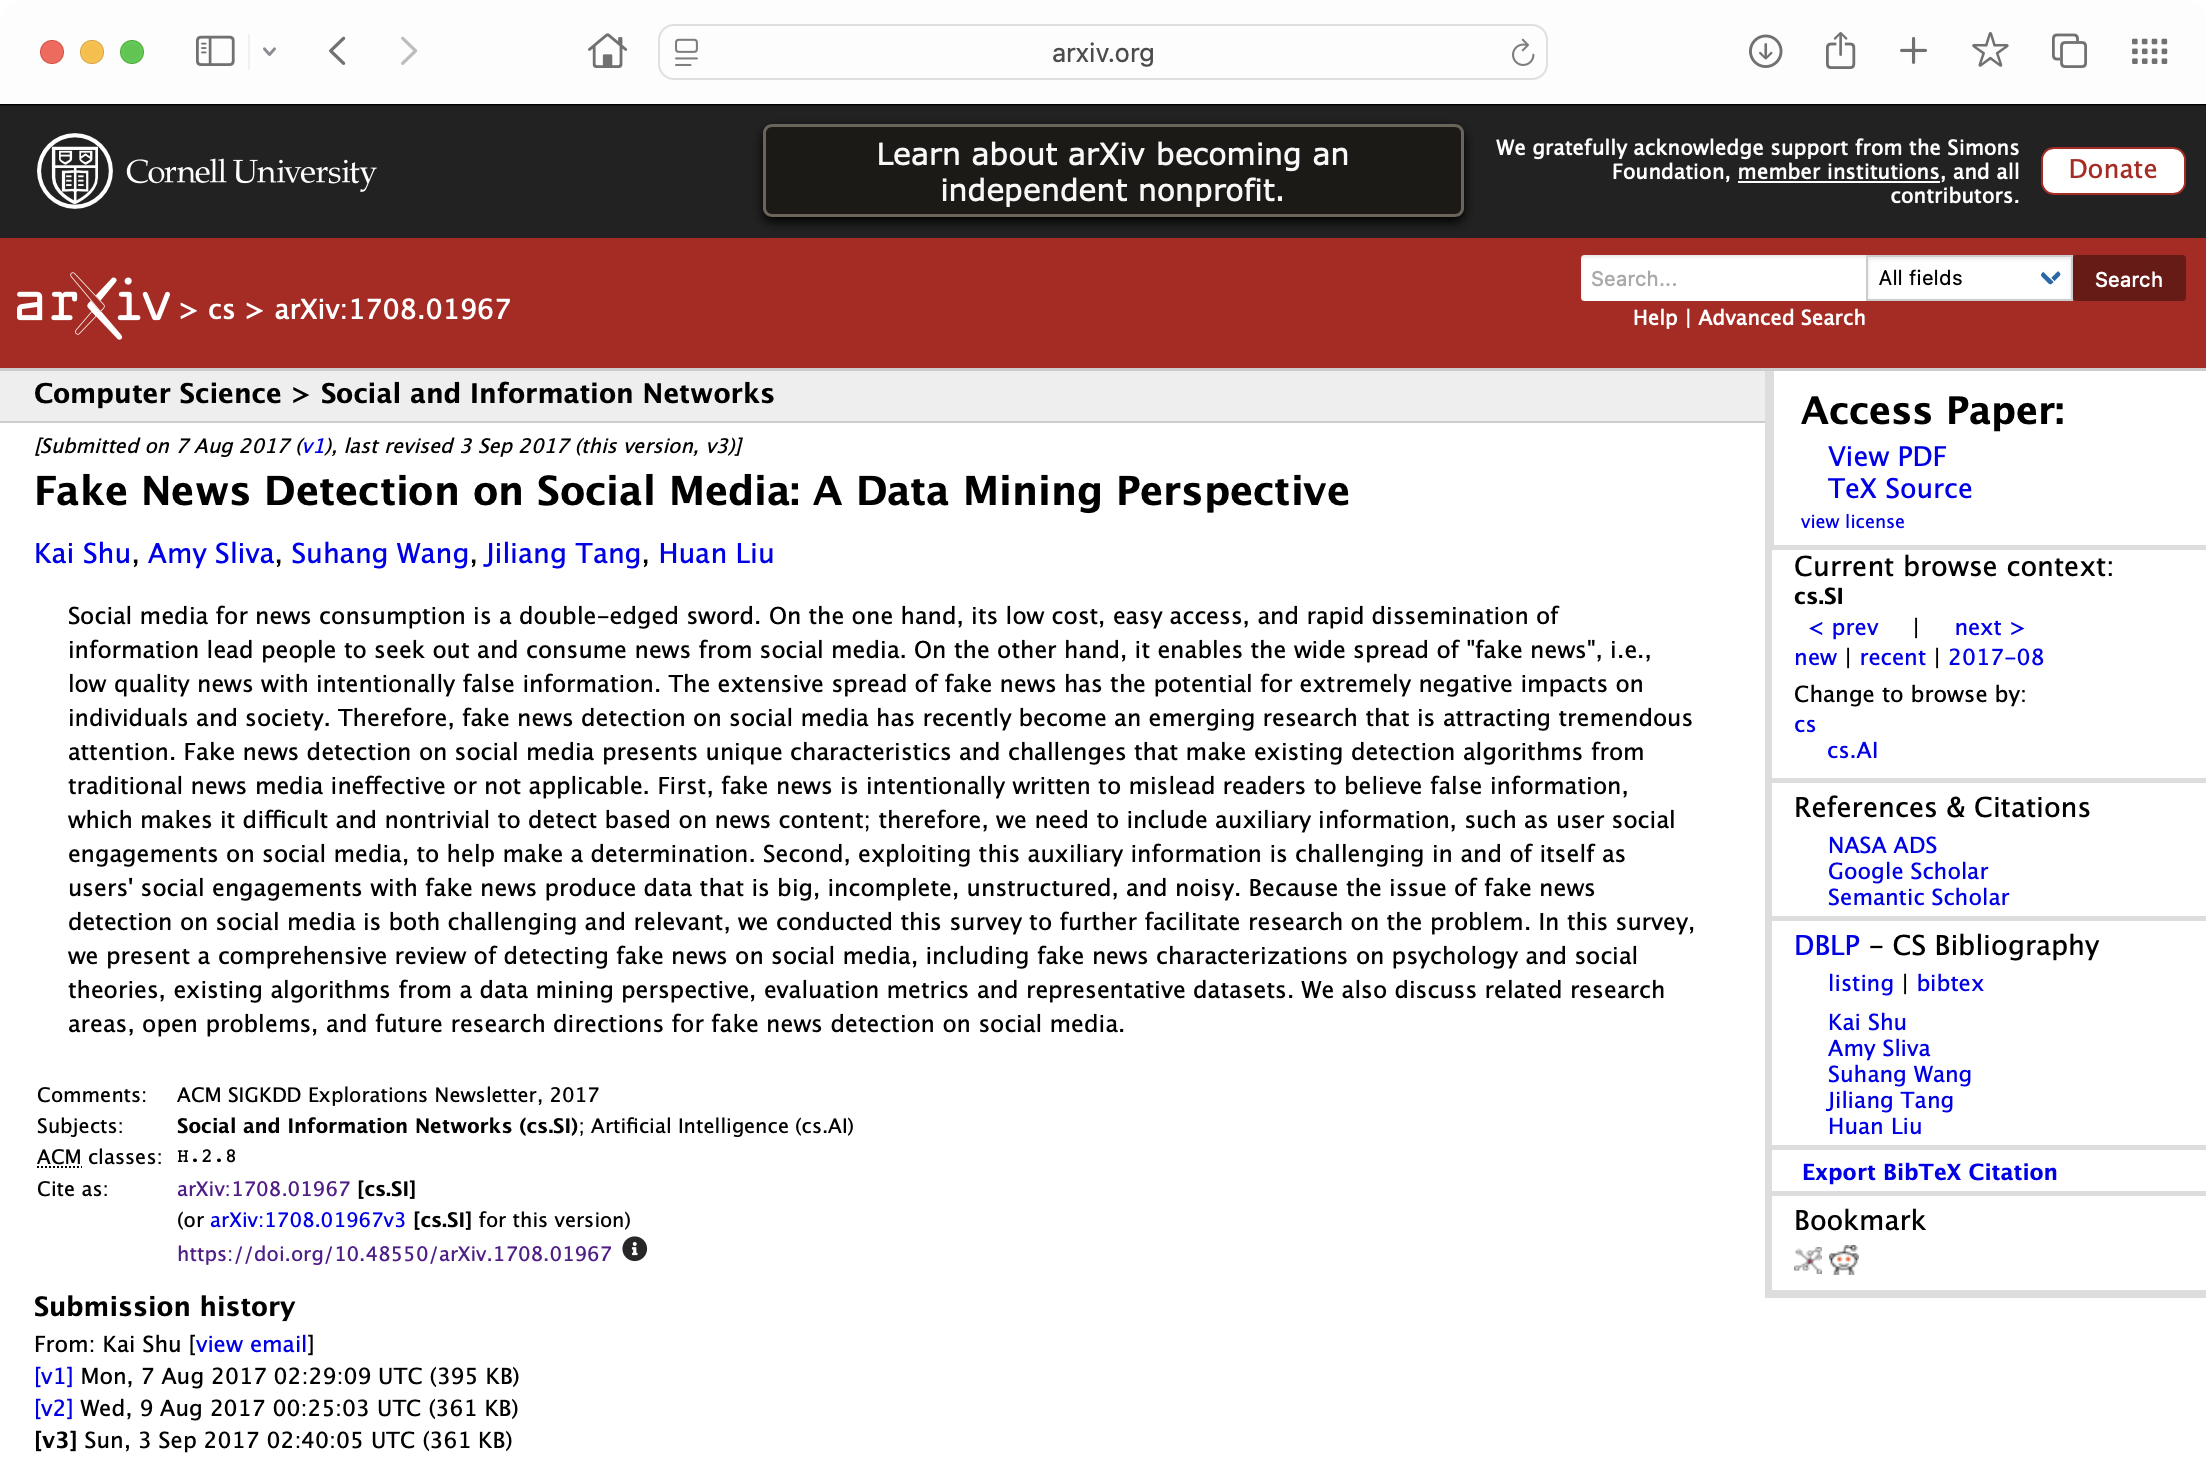
\includegraphics[height=.75\textheight]{Screenshot 2026-05-22 at 5.13.47 PM}
{\footnotesize \url{https://arxiv.org/abs/1708.01967} for details.}
\end{frame}

%-----------------------------------------------
\begin{frame}{}
\begin{block}{Framework}
\vspace{.4cm}
\centering
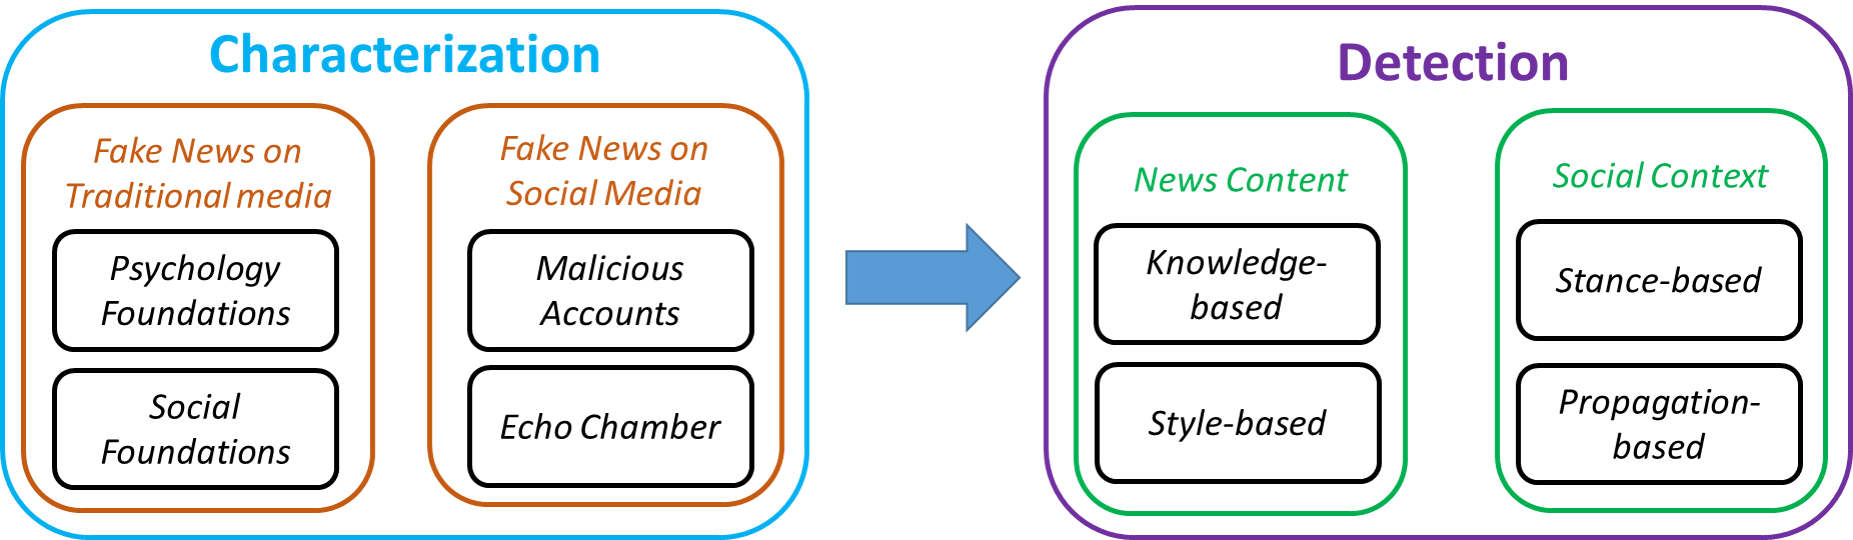
\includegraphics[height=3cm]{framework.png}
{\footnotesize \url{https://arxiv.org/abs/1708.01967} for details.}
\end{block}
\end{frame}

%-----------------------------------------------
\begin{frame}{}
\begin{block}{Future Directions}
\vspace{.4cm}
\centering
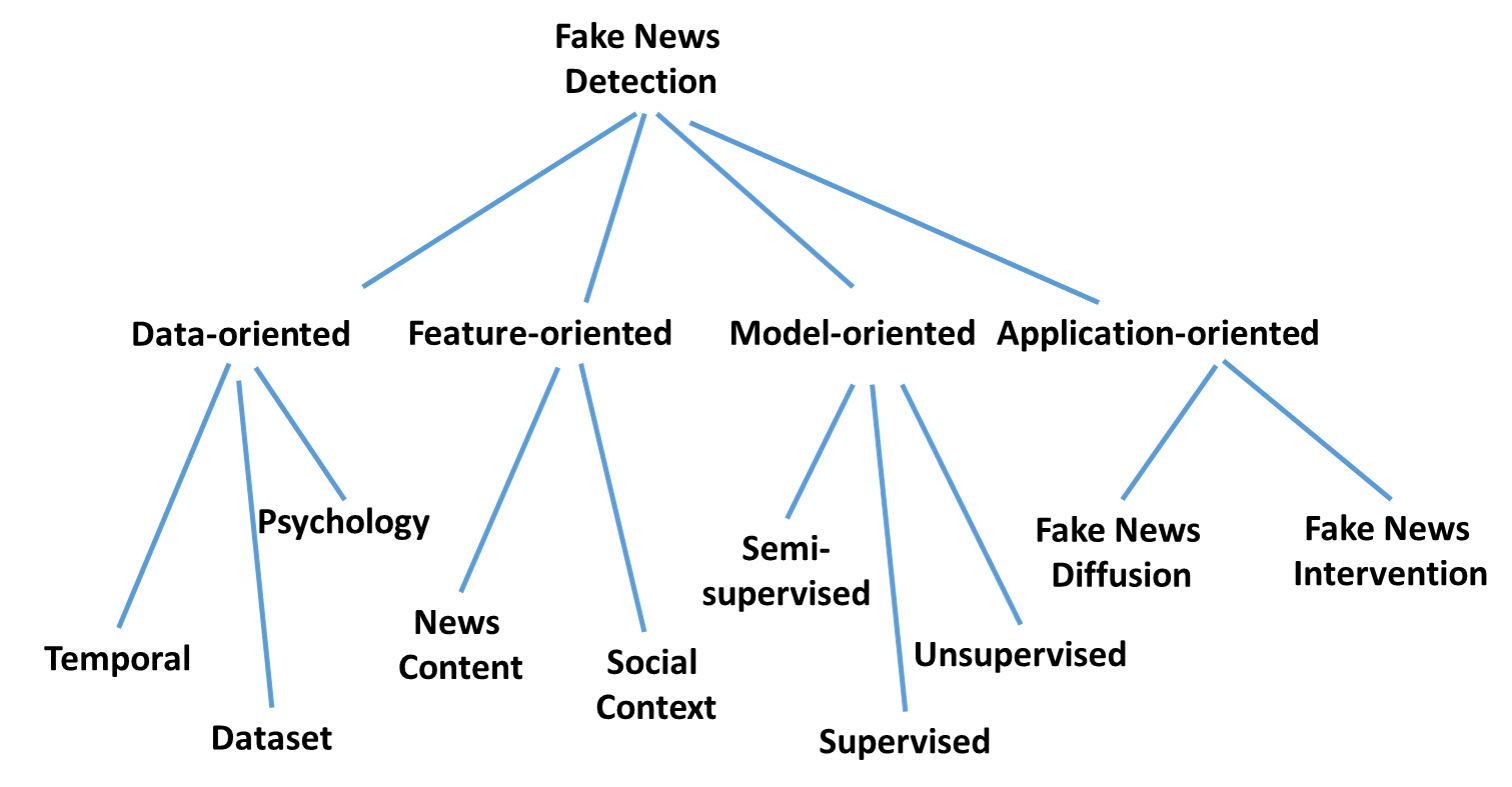
\includegraphics[height=5.5cm]{future_direction.png}
{\footnotesize \url{https://arxiv.org/abs/1708.01967} for details.}
\end{block}
\end{frame}

%-----------------------------------------------
\begin{frame}{Building a Bayesian Model for Events}
Before reading anything,\\we can use prior knowledge from historical data.
\vspace{0.8cm}
\begin{block}{Valid Probability Model}
A probability model must satisfy:
\pause
\begin{enumerate}
\item Cover all possible events.
\item Assign probabilities to each event.
\item Probabilities sum to one.
\end{enumerate}
\end{block}
\end{frame}

{
\setbeamercolor{background canvas}{bg=green!10}
%-----------------------------------------------
\begin{frame}{We’re Using \texttt{R} Instead of Python}
\begin{block}{Python}
\begin{itemize}
\item "Can do everything" ... installs $n$ packages, breaks after update
\item Stack Overflow becomes your TA
\end{itemize}
\end{block}
\begin{block}{\texttt{R} \quad \rightarrow \quad \url{https://cran.r-project.org}}
\begin{itemize}
\item Literally for statistics; \hl{\texttt{lm(y \textasciitilde{} x)}} and \ul{move on} with your life
\item Excellent, open-source, keeps us focused on data analysis,\\... and I enjoy sleeping at night!
\end{itemize}
\end{block}
\mbox{\textbf{What I Need From You:} learn concepts, analyze data, pass the class!}\\
\textbf{What I Do Not Need:} a 2-hour debate about virtual environments.
\end{frame}
}

%-----------------------------------------------
\begin{frame}[fragile]{}

\begin{columns}[t]
\begin{column}{0.285\textwidth}
\begin{block}{Dataset}
\begin{minted}[fontsize=\footnotesize, linenos]{r}
# Load packages
library(bayesrules)
library(tidyverse)
library(janitor)

# Import article data
data(fake_news)

fake_news %>% 
tabyl(type) %>% 
adorn_totals("row")
#  type   n percent
#  fake  60     0.4
#  real  90     0.6
# Total 150     1.0
\end{minted}
\end{block}
\end{column}

\begin{column}{0.53\textwidth}
\begin{block}{Prior Probability Model}
\begin{itemize}
\item 150 news articles:\\60 fake, 90 real
\item $P(\text{Fake}) = \frac{60}{150} = 0.40$.\\
  Before looking at the headline, the prior probability that an article is fake is 40\%.
\end{itemize}
\end{block}
\end{column}
\end{columns}
\end{frame}

%-----------------------------------------------
\begin{frame}{}
\textbf{Prior Belief}: there is a 40\% chance an article is fake before observing any evidence.
\[
P(B)=0.40 \quad \leftrightarrow \quad P(B^c)=0.60
\]
where \(B\): article is \textbf{fake}, \(B^c\): article is \textbf{real}.
\vspace{0.2cm}
\[
P(B) + P(B^c) = 0.40 + 0.60 = 1
\]
\begin{center}
\begin{tabular}{c|ccc}
\textbf{Event} & \(B\) & \(B^c\) & Total \\
\hline
Probability & 0.4 & 0.6 & 1
\end{tabular}
\end{center}
\end{frame}

%-----------------------------------------------
\begin{frame}{}
\begin{block}{}
Bayesian reasoning to estimate whether a news article is fake:
\vspace{0.8em}

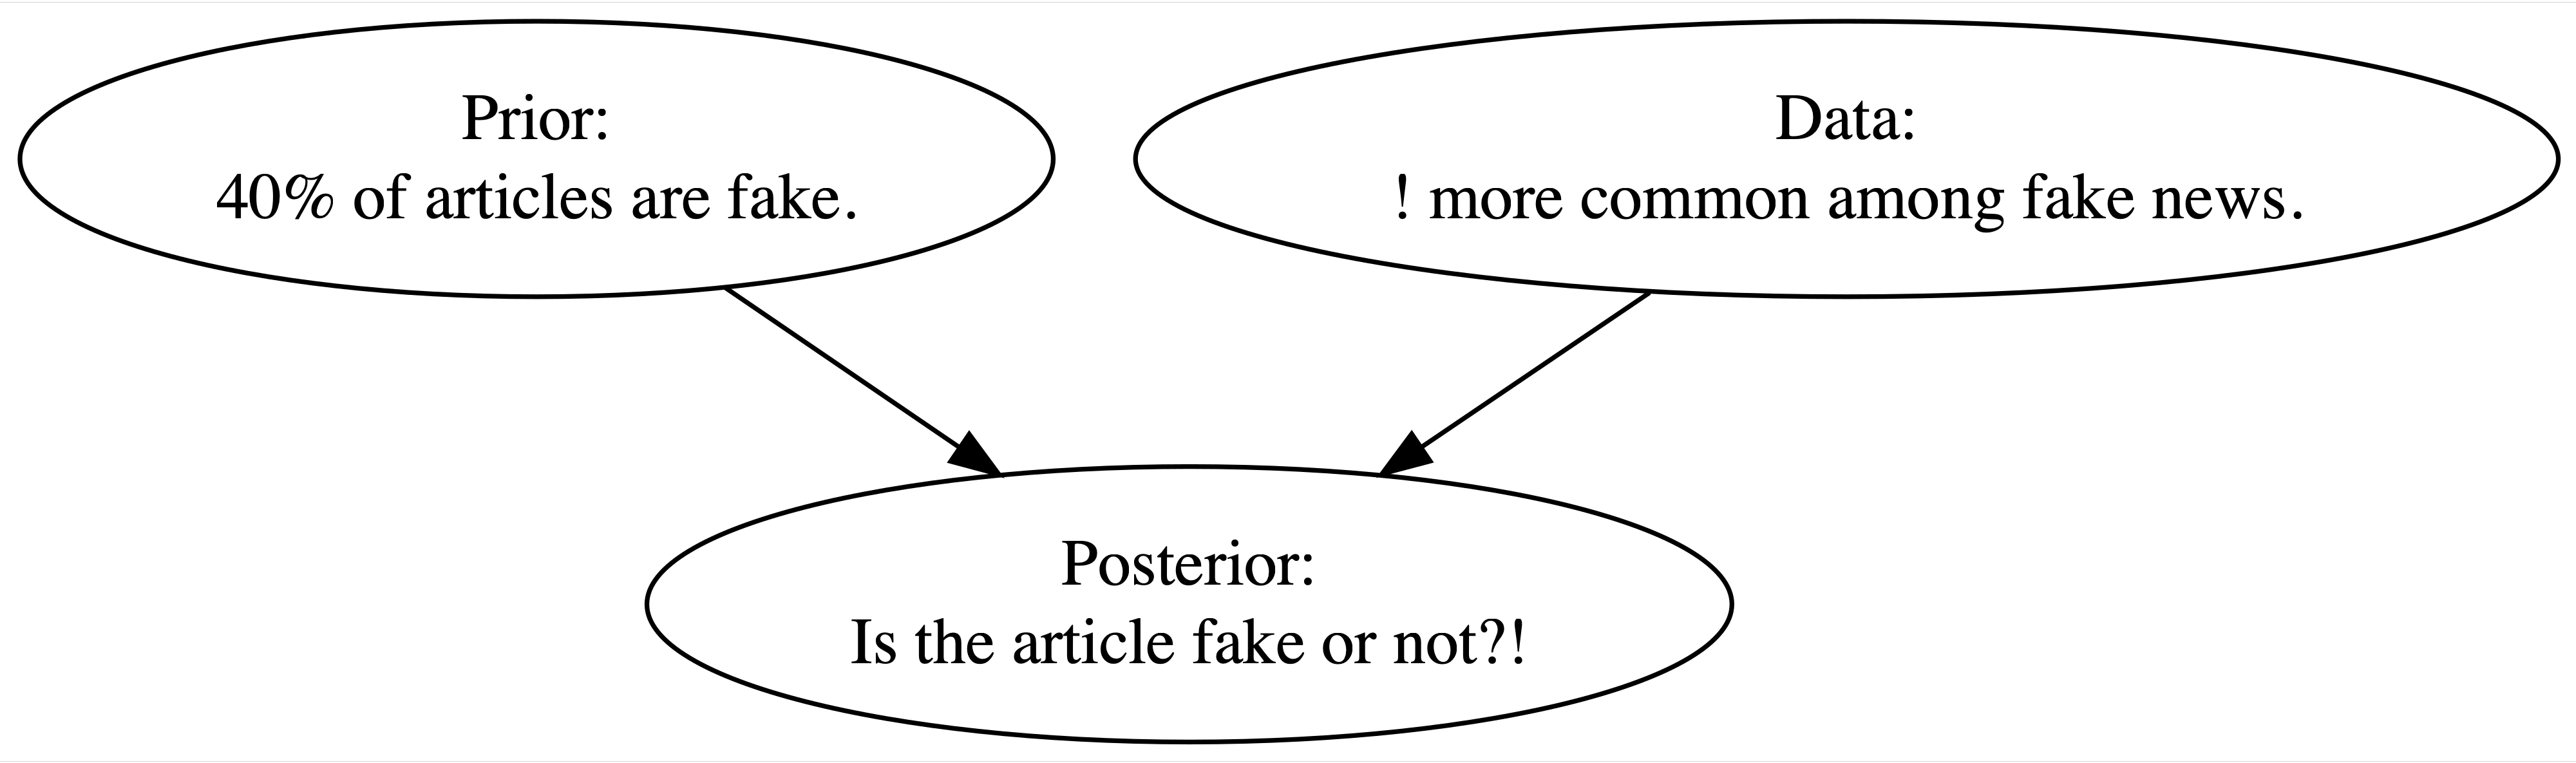
\includegraphics[height=3.3cm]{fake_news_diagram.png}
\end{block}
\end{frame}

%-----------------------------------------------
\begin{frame}{}
\begin{block}{DAG: Directed Acyclic Graph}
\begin{center}
\begin{tikzpicture}[
node distance=3cm,
every node/.style={circle, draw, thick, minimum size=1.3cm}
]
\node (A) {\(A\)};
\node[right of=A] (B) {\(B\)};
\draw[-Triangle, thick] (A) -- (B);
\end{tikzpicture}
$
A = \text{exclamation points "!"}
\quad
\quad
B = \text{fake status "\emoji{disguised-face}"}$
\end{center}
\begin{itemize}
\item A \textbf{DAG} shows how variables are connected.
\item The arrow means \(A\) may be associate with \(B\).
\item \textbf{Acyclic} means the arrows do not loop back.
\end{itemize}
\end{block}
\end{frame}

%-----------------------------------------------
\begin{frame}{}
\begin{block}{DAGs and Conditional Probability}
\begin{itemize}
\item The DAG suggests that the chance of \(B\) may depend on \(A\).
\[
P(B \mid A)
\]
\item[] In words: the probability of article is fake \textbf{given}\\
    \hspace{4cm}the exclamation point in the title.
\pause
\item If \(A\) changes the probability of \(B\),\\
  \hspace{2cm}then the events are \textbf{dependent}.
\[
P(B \mid A) \neq P(B)
\]
\item \pause If knowing \(A\) does not change the probability of \(B\),\\
  \hspace{5cm}then they are \textbf{independent}.
\[
P(B \mid A) = P(B)
\]
\end{itemize}
\end{block}
\end{frame}

%-----------------------------------------------
\begin{frame}[fragile]{}
\begin{minted}[fontsize=\footnotesize, linenos]{r}
# Transposed version of head()
# ... makes possible to see all columns in a data frame
glimpse(fake_news)
\end{minted}

\vspace{1.em}

Observed headline pattern:

\begin{minted}[fontsize=\footnotesize, linenos]{r}
# Tabulate exclamation usage and article type
fake_news %>% 
tabyl(title_has_excl, type) %>% 
adorn_totals("row")
# title_has_excl fake real
#          FALSE   44   88
#           TRUE   16    2
#          Total   60   90
\end{minted}
\end{frame}

%------------------------------------------------
\begin{frame}{}

\begin{textblock*}{2cm}(11cm,0.3cm)

\includegraphics[width=1.5cm]{bookmark.png}
\end{textblock*}

\href{https://abuabara.github.io/DAEN427F26/Lecture2.R}{Code: https://abuabara.github.io/DAEN427F26/Lecture2.R}
\end{frame}

%-----------------------------------------------
\begin{frame}{}
\begin{block}{Exclamation Points as Evidence}

\vspace{0.4em}
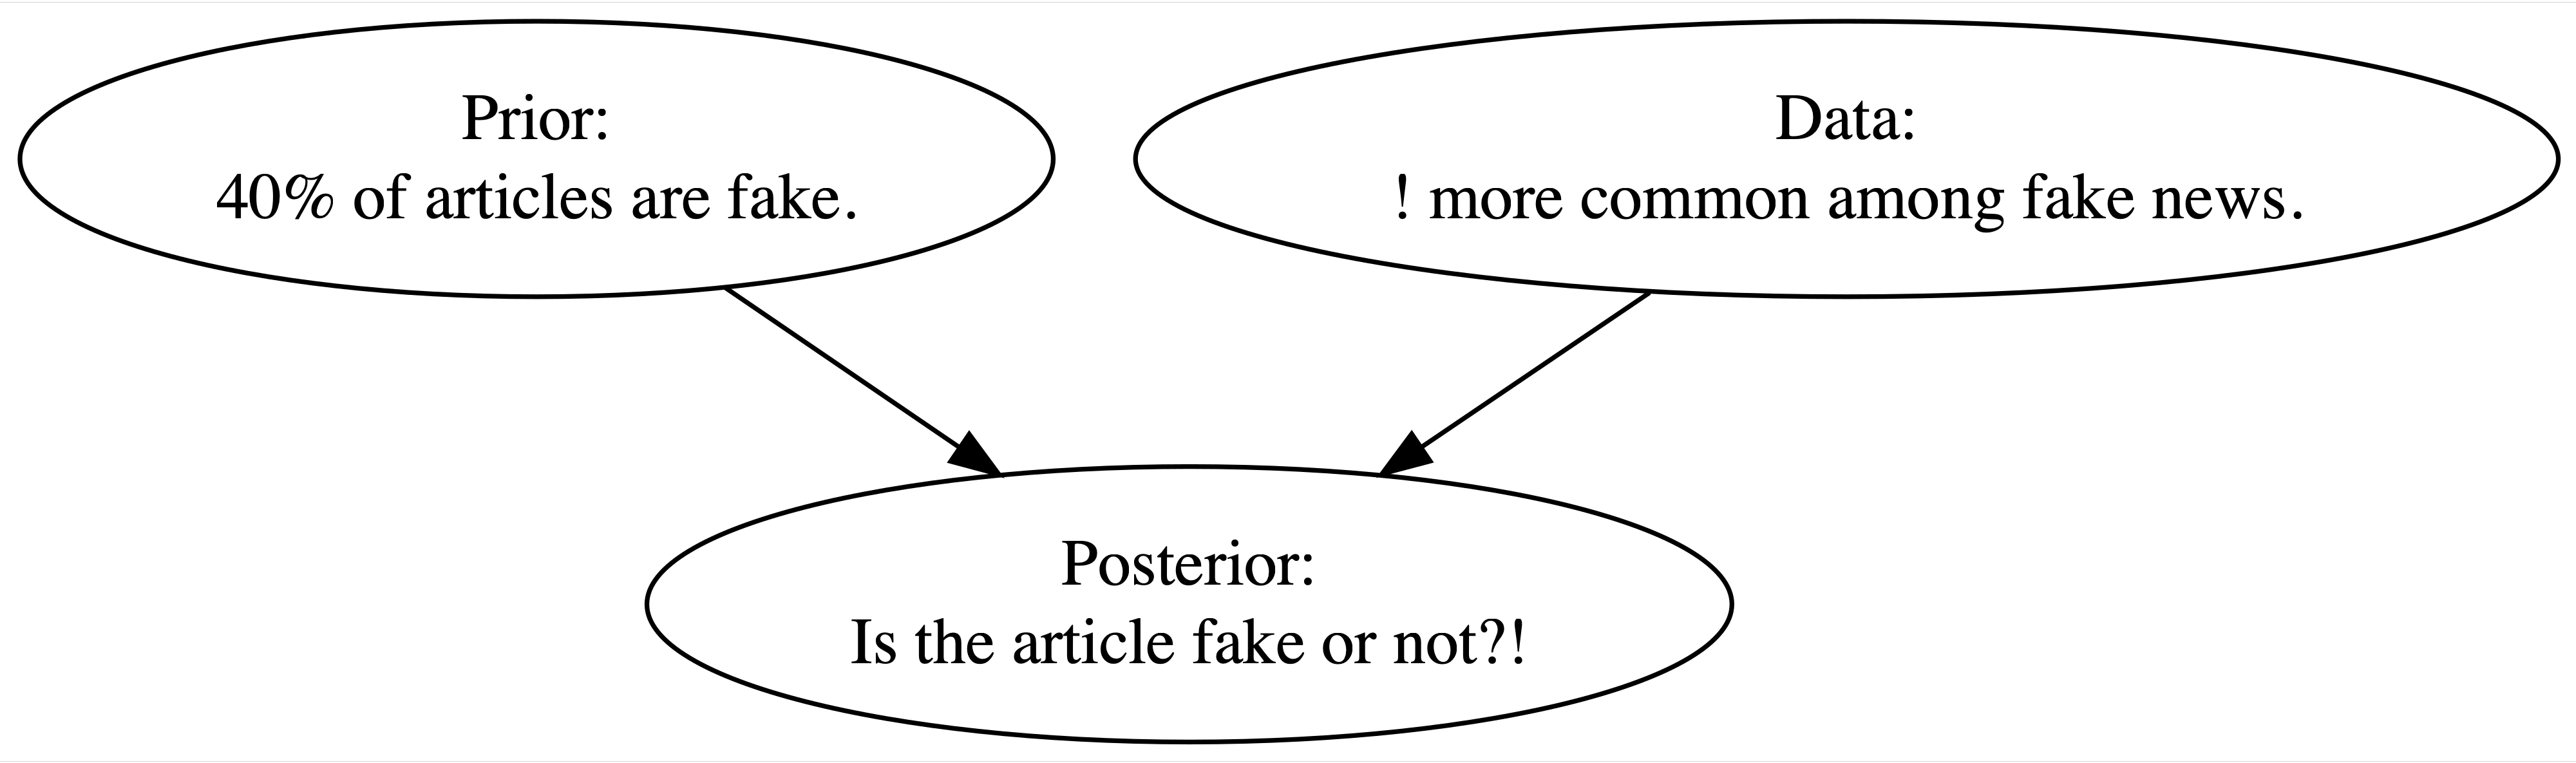
\includegraphics[height=3.4cm]{fake_news_diagram.png}
\begin{table}
\centering
\begin{tabular}{lrrr}
\toprule
\textbf{Title Has ``!''} & \textbf{Fake} & \textbf{Real} & \textbf{Total} \\
\midrule
Yes & 16 & 2  & 18 \\
No  & 44 & 88 & 132 \\
\midrule
Total & 60 & 90 & 150 \\
\bottomrule
\end{tabular}
\end{table}
\end{block}
\end{frame}

%-----------------------------------------------
\begin{frame}{}
\begin{block}{Conditional Probability \& Likelihood}
\begin{table}
\centering
\begin{tabular}{lrrr}
\toprule
\textbf{Title Has ``!''} & \textbf{Fake} & \textbf{Real} & \textbf{Total} \\
\midrule
Yes & 16 & 2  & 18 \\
No  & 44 & 88 & 132 \\
\midrule
Total & 60 & 90 & 150 \\
\bottomrule
\end{tabular}
\end{table}
\begin{center}
$P(! \mid \text{Fake}) = \frac{16}{60} \approx 0.267$,
$P(! \mid \text{Real}) = \frac{2}{90} \approx 0.022$
\end{center}
\vspace{0.4em}
An exclamation point increases the probability that an article \hl{is fake}.
\end{block}
\end{frame}

%-----------------------------------------------
\begin{frame}{}
\begin{block}{Conditional Probability \& Likelihood}
\[
\begin{aligned}
B &: \text{article is fake} \\
B^c &: \text{article is real}
\end{aligned}
\]
\[
\begin{aligned}
A &: \text{article uses exclamation points} \\
A^c &: \text{article does not use exclamation points}
\end{aligned}
\]
From the data:
\[
P(A \mid B)=0.267 \qquad P(A \mid B^c)=0.022
\]
Fake news articles are \textbf{much more likely} to use exclamation points than real news articles.
\end{block}
\end{frame}

%-----------------------------------------------
\begin{frame}{}
\begin{block}{Conditional vs Unconditional Probability}
\begin{itemize}
\item \textbf{Unconditional probability} is the chance something happens without extra information.
\[
P(A)
\]
\item \textbf{Conditional probability} is the chance something happens given that something else is already known.
\[
P(A \mid B)
\]
\item Comparing \(P(A)\) and \(P(A \mid B)\) tells us whether knowing \(B\) changes how likely \(A\) is.
\end{itemize}
\end{block}
\end{frame}

%-----------------------------------------------
\begin{frame}{}
\begin{block}{Independent Events}
\begin{itemize}
\item Two events are \textbf{independent} if knowing one happens does not change the probability of the other.
\item \textcolor{aggiemaroon!70}{\emph{Example}: rolling a die and flipping a coin are independent, because the die result \textbf{does not} affect the coin flip.}
\item In symbols:
\[
P(A \mid B) = P(A)
\]
\end{itemize}
\end{block}
\end{frame}

%-----------------------------------------------
\begin{frame}{}
\begin{block}{From Probability to Likelihood}
\begin{itemize}
\item Earlier, we computed:
\[
P(A \mid B)=0.2667
\qquad
P(A \mid B^c)=0.0222
\]
\item Fake articles are much more likely to use exclamation points.
\item Suppose we already observed an article with exclamations.
\item[] Now the question becomes:\\
  \centering \textit{Is the article more likely fake or real?}
\end{itemize}
\end{block}
\end{frame}

%-----------------------------------------------
\begin{frame}{}
\begin{block}{What is Likelihood?}
\begin{itemize}
\item \textbf{Probability} starts with a known cause and predicts data.
\[
P(A \mid B)
\]
\item \textbf{Likelihood} starts with observed data and compares possible causes.
\[
\mathcal{L}(B \mid A)=P(A \mid B)
\]
\item In our example:
\begin{itemize}
\item \(A\): article uses exclamation points
\item \(B\): article is fake
\item Since
      \[
      P(A \mid B) > P(A \mid B^c)
      \]
      \emph{exclamation} provide evidence that the article may be fake.
\end{itemize}
\end{itemize}
\end{block}
\end{frame}

%-----------------------------------------------
\begin{frame}{}
\begin{center}
\begin{tabular}{p{4cm}|p{4cm}}
\textbf{Probability} & \textbf{Likelihood} \\
\hline
Known condition & Known data \\
Predicts outcomes & Compares explanations \\
\[
P(A \mid B)
\]
& 
\[
\mathcal{L}(B \mid A)
\]
\end{tabular}
\end{center}
\begin{itemize}
\item The distinction is \textbf{subtle}, especially since people use the terms “likelihood” and “probability” interchangeably in casual conversation.
\item Likelihood \textbf{helps us decide} which explanation best fits the observed data.
\end{itemize}
\end{frame}

%-----------------------------------------------
\begin{frame}{}

\begin{block}{}
\begin{itemize}
\item The likelihood function \textbf{is not} a probability function, but rather provides a framework to compare the relative compatibility of our exclamation point data with $B$ and $B^c$.
\end{itemize}
\begin{table}[h]
\centering
\begin{tabular}{lccc}
\hline
\textbf{Event}              & \(B\)  & \(B^c\) & \textbf{Total} \\
\hline
Prior probability           & 0.4    & 0.6     & 1              \\[0.1cm]
Likelihood $(\cdot \mid A)$ & 0.2667 & 0.0232  & \hl{0.2889}    \\
\hline
\end{tabular}
\end{table}
\end{block}
\end{frame}

{
\setbeamercolor{background canvas}{bg=blue!10}
%-----------------------------------------------
\begin{frame}{}
\begin{block}{Quiz}
Two boxes are available:

\begin{itemize}
\item Box 1 contains 4 red and 2 green balls.
\item Box 2 contains 2 red and 4 green balls.
\item The probability of choosing either box is equal:
\[
P(E_1)=P(E_2)=\frac12.
\]
\item A box is selected at random, and one ball is drawn.
\item Study the \textbf{likelihood} of observing a red ball under each box.
\end{itemize}
\end{block}
\end{frame}

%-----------------------------------------------
\begin{frame}{}
\begin{block}{}
\begin{center}
\begin{tikzpicture}[scale=1]

% Outer rectangle
\draw[thick] (0,0) rectangle (10,5);

% Divider
\draw[thick] (5.,0) -- (5.,5);

% Labels
% \node at (2.3,5.4) {$B1$};
% \node at (7.7,5.4) {$B2$};

% Left side label
\node at (0.8,4.2) {$B_1$};

% Right side label
\node at (9.2,4.2) {$B_2$};

% Red ellipse
\draw[red, thick] (4.75,2.5) ellipse (3.2 and 1.2);
\node[red] at (6.9,2.0) {$R$};

% Left box red balls
\fill[red] (2.7,3.0) circle (0.12);
\fill[red] (3.8,3.0) circle (0.12);
\fill[red] (2.1,2.2) circle (0.12);
\fill[red] (3.3,1.7) circle (0.12);

% Left box green balls
\fill[green!70!black] (1.4,3.8) circle (0.12);
\fill[green!70!black] (0.7,2.5) circle (0.12);

% Right box red balls
\fill[red] (6.5,2.7) circle (0.12);
\fill[red] (5.9,1.8) circle (0.12);

% Right box green balls
\fill[green!70!black] (7.4,3.9) circle (0.12);
\fill[green!70!black] (8.8,3.2) circle (0.12);
\fill[green!70!black] (8.9,1.5) circle (0.12);
\fill[green!70!black] (6.7,0.9) circle (0.12);

\end{tikzpicture}
\end{center}
\end{block}
\end{frame}

%-----------------------------------------------
\begin{frame}{}
\begin{block}{}
\small
\textbf{Answer:}
{\color{blue}
A red ball is more consistent with Box 1 than with Box 2.\\[.1cm]

The likelihoods are:
$P(R\mid B_1)=\frac46=\frac23$
and
$P(R\mid B_2)=\frac26=\frac13.$\\[.1cm]

So, if Box 1 had been selected, observing a red ball would be more likely.

\begin{center}
$P(R\mid B_1) > P(R\mid B_2)$
\end{center}

Therefore, the red ball provides stronger evidence for Box 1 than for Box 2.
\[
\frac{P(R\mid B_1)}{P(R\mid B_2)} = \frac{\frac23}{\frac13} = 2
\]
The observed red ball is \textbf{twice} as likely under Box 1 as under Box 2. Since the boxes were equally likely before the draw, the red ball favors Box 1.
}
\end{block}
\end{frame}
}

%-----------------------------------------------
\begin{frame}{}
\begin{block}{Recap}
\[
\begin{aligned}
&A   = \text{article uses exclamation points}\\
&A^c = \text{article does not use exclamation points}\\
&B    = \text{article is fake news}\\
&B^c  = \text{article is real news}
\end{aligned}
\]
\vspace{0.2cm}

From the prior model:
\[
P(B)=0.4
\qquad
P(B^c)=0.6
\]

So, 40\% of articles are fake and 60\% are real.
\end{block}
\end{frame}

%-----------------------------------------------
\begin{frame}{}

\begin{textblock*}{2cm}(11cm,0.3cm)

\includegraphics[width=1.5cm]{bookmark.png}
\end{textblock*}

\begin{block}{Normalizing Constants}
\begin{itemize}
\item The marginal probability of observing exclamation points across all articles is $P(A)$.
\item This is called the \textbf{normalizing constant}.
%    \pause
\item To calculate it, we split articles into two groups:\\
  \hspace{2cm}$P(A)=P(A \cap B)+P(A \cap B^c)$
\item That is:\\ \mbox{$\text{Exclamations} = \text{fake with exclamations} + \text{real with exclamations}$}
\end{itemize}
\end{block}
\end{frame}

%-----------------------------------------------
\begin{frame}{}
\begin{block}{Joint Probability Table}
\[
\begin{array}{c|ccc}
& B & B^c & \text{Total} \\
\hline
A & P(A \cap B) & P(A \cap B^c) & P(A) \\
A^c & P(A^c \cap B) & P(A^c \cap B^c) & P(A^c) \\
\hline
\text{Total} & 0.4 & 0.6 & 1
\end{array}
\]
\vspace{0.2cm}
\begin{itemize}
\item Each inside cell is a \textbf{joint probability}.
\item For example: $P(A \cap B)$ means the probability that an article is fake and uses exclamation points.
\end{itemize}
\end{block}
\end{frame}

%-----------------------------------------------
\begin{frame}{}
\begin{block}{Fake Articles \textbf{with} Exclamation Points}
\begin{itemize}
\item To determine the probabilities of these joint events, note that 40\% of articles are fake and 26.67\% of fake articles use exclamation points, $P(B) = 0.4$ and $P(A \mid B) = 0.2667$. 
\item The joint probability is
$P(A \cap B) = P(A \mid B) ~ P(B) = 0.2667 \cdot 0.4 = 0.1067$
\item So, 10.67\% of all articles are fake and use exclamation points.
\end{itemize}
\end{block}
\end{frame}

%-----------------------------------------------
\begin{frame}{}
\begin{block}{}
\[
\begin{array}{c|ccc}
& B & B^c & \text{Total} \\
\hline
A & $0.4 \cdot 16/60 = \textbf{0.107}$ & P(A \cap B^c) & $32/150 = 0.12$ \\
A^c & P(A^c \cap B) & P(A^c \cap B^c) & $118/150 = 0.78$ \\
\hline
\text{Total} & \textbf{0.4} & 0.6 & 1
\end{array}
\]
\end{block}
\end{frame}

%-----------------------------------------------
\begin{frame}{}
\begin{block}{Fake Articles \textbf{without} Exclamation Points}
\begin{itemize}
\item Since 26.67\% of fake articles use exclamation points, $1 - 0.2667 = 73.33\%$ do not use exclamation points.
\item Then, $P(A^c \cap B) = P(A^c\mid B)~P(B) = 0.7333 \cdot 0.4 = 0.2933$
\item So, 29.33\% of all articles are fake and do not use exclamation.
\end{itemize}
\end{block}
\end{frame}

%-----------------------------------------------
\begin{frame}{}
\begin{block}{Checking the Fake Article Total}
The fake-news column is split into two parts:

\[P(A \cap B) \quad \text{and} \quad P(A^c \cap B)\]

Therefore,
\[
P(B)=P(A \cap B)+P(A^c \cap B)
\]
\[
P(B)=0.1067+0.2933
\]
\[
P(B)=0.4
\]

This matches the prior probability that an article is fake.
\end{block}
\end{frame}

%-----------------------------------------------
\begin{frame}{}
\begin{block}{Real Articles}
From the likelihood function: $P(A\mid B^c)=0.0222$\\

So only 2.22\% of real articles use exclamation points.\\

The joint probability is
\[
P(A \cap B^c)=P(A\mid B^c)P(B^c)
\]
\[
P(A \cap B^c)=0.0222 \cdot 0.6
\]
\[
P(A \cap B^c)=0.0133
\]

So, 1.33\% of all articles are real and use exclamation points.
\end{block}
\end{frame}

%-----------------------------------------------
\begin{frame}{}
\begin{block}{Real Articles without Exclamation Points}
Since
\[
P(A\mid B^c)=0.0222
\]
we have
\[
P(A^c\mid B^c)=1-0.0222
\]
\[
P(A^c\mid B^c)=0.9778
\]

Then
\[
P(A^c \cap B^c)=P(A^c\mid B^c) ~ P(B^c)
\]
\[
P(A^c \cap B^c)=0.9778 \cdot 0.6
\]
\[
P(A^c \cap B^c)=0.5867
\]
\end{block}
\end{frame}

%-----------------------------------------------
\begin{frame}{}
\begin{block}{Completed Joint Probability Table}
\[
\begin{array}{c|ccc}
& B & B^c & \text{Total} \\
\hline
A   & 0.107 & 0.013 & 0.12 \\
A^c & 0.293 & 0.587 & 0.88 \\
\hline
\text{Total} & 0.4 & 0.6 & 1
\end{array}
\]

The row total for \(A\) gives the \textbf{normalizing constant}:
\[
P(A) = 0.107 + 0.013 = \boxed{0.12}
\]

So, 12\% of all articles use exclamation points.
\end{block}
\end{frame}

%-----------------------------------------------
\begin{frame}{}
\begin{block}{Joint Probability}
The calculations use the relationship
\[
P(A \cap B)=P(A\mid B)P(B)
\]

This connects: $~ \text{joint probability}$\\

with: $~ \text{conditional probability} \times \text{prior probability}$\\

Rearranging gives the conditional probability formula:
\[
P(A\mid B)=\frac{P(A \cap B)}{P(B)}
\]

\textcolor{aggiemaroon!70}{
PS. If \(A\) and \(B\) are \textbf{independent}, then:
$P(A \cap B) = P(A) ~ P(B)$
}
\end{block}
\end{frame}


%-----------------------------------------------
\begin{frame}{}
\begin{block}{
Representation of Conditional Probability
}
\begin{figure}[h]
\centering
\[
P(A\mid B)
=
\frac{P(A\cap B)}{P(B)}=
\frac{
\begin{tikzpicture}[baseline=-0.5ex,scale=0.8]
% Rectangle
\draw (0,0) rectangle (4,2);

% Circles
\begin{scope}
\clip (1.2,1) circle (0.8);
\fill[AggieMaroon!35] (2.4,1) circle (0.8);
\end{scope}

\draw (1.2,1) circle (0.8);
\draw (2.4,1) circle (0.8);

\node at (0.75,1) {$A$};
\node at (2.8,1) {$B$};
\end{tikzpicture}
}
{
\begin{tikzpicture}[baseline=-0.5ex,scale=0.8]
% Rectangle
\draw (0,0) rectangle (4,2);

% Event B
\fill[AggieMaroon!35] (2.4,1) circle (0.8);

\draw (1.2,1) circle (0.8);
\draw (2.4,1) circle (0.8);

\node at (0.75,1) {$A$};
\node at (2.8,1) {$B$};
\end{tikzpicture}
}
\]
\end{figure}
\end{block}
\end{frame}

%-----------------------------------------------
\begin{frame}{}
\begin{block}{Conditional Probability}
Conditional probability answers the question:
\[
\textit{“What is the probability of } A \textit{ given that } B \textit{ has occurred?”}
\]

The definition is:
\[
P(A \mid B) = \frac{P(A \cap B)}{P(B)}
\qquad \text{where } P(B) \neq 0
\]

\begin{itemize}
\item Start with the probability that both \(A\) and \(B\) occur
\item Restrict attention only to situations where \(B\) occurs
\item Measure how often \(A\) also occurs
\end{itemize}
\vspace{0.4cm}

\textcolor{aggiemaroon!70}{
\textbf{Example:}
$
P(\text{Rain} \mid \text{Cloudy})
=
\frac{
P(\text{Rain and Cloudy})
}{
P(\text{Cloudy})
}
$
}
\end{block}
\end{frame}

%-----------------------------------------------
\begin{frame}{}
\begin{block}{Law of Total Probability}
Suppose event \(A\) can happen in two distinct ways:
\[
A \cap B
\qquad \text{or} \qquad
A \cap B^c
\]

Since \(B\) and \(B^c\) cover all possibilities, we can write:
\[
P(A) = P(A \cap B) + P(A \cap B^c)
\]

Using the joint probability rule:
\[
P(A \cap B) = P(A \mid B)P(B)
\]

we get the \textbf{Law of Total Probability}:
\[
P(A)
=
P(A \mid B)P(B)
+
P(A \mid B^c)P(B^c)
\]
\end{block}
\end{frame}

%-----------------------------------------------
\begin{frame}{}
\begin{block}{Exclamation Points in News Articles}
\[
\begin{aligned}
A &= \text{article uses an exclamation point}\\
B &= \text{article is fake news}
\end{aligned}
\]

\[
P(A \mid B)=0.2667,
\qquad
P(B)=0.4
\]
\[
P(A \mid B^c)=0.0222,
\qquad
P(B^c)=0.6
\]
Then:
\[
P(A)
=
0.2667~(0.4) + 0.0222~(0.6)
\]
\[
P(A)
=
0.1067 + 0.0133
=
0.12
\]\\
So, about \textbf{12\% of all articles} use exclamation points.
\end{block}
\end{frame}

%-----------------------------------------------
\begin{frame}{}
\begin{block}{}
\[
\begin{array}{c|ccc}
& B & B^c & \text{Total} \\
\hline
A   & 0.107 & 0.013 & 0.12 \\
A^c & 0.293 & 0.587 & 0.88 \\
\hline
\text{Total} & 0.4 & 0.6 & 1
\end{array}
\]

\[
P(A) = 0.107 + 0.013 = \boxed{0.12}
\]

\end{block}
\end{frame}

{
\setbeamercolor{background canvas}{bg=orange!10}
%-----------------------------------------------
\begin{frame}{Homework}
\begin{itemize}
\color{aggiemaroon}{
\item Questions 1–5 next; questions 6-9 at the end of the topic.
\item Submit all answers by Fri Sep 11.
\item You may discuss with peers but submissions must be individual.
\item Responses may be shared anonymously during class discussion!
}
\end{itemize}
\end{frame}

%-----------------------------------------------
\begin{frame}{}
\begin{block}{Question 1}
\small
For each scenario below, you’re given a pair of events, $A$ and $B$.
Explain what you believe to be the relationship between the posterior and prior probabilities of $B$: $P(B | A) > P(B)$ or $P(B | A) < P(B)$.:
\begin{enumerate}
\item[a)] $A =$ you just finished reading Lambda Literary Award-winning author Nicole Dennis-Benn’s first novel, and you enjoyed it!\\
$B =$ you will also enjoy Benn’s newest novel.
\item[b)] $A =$ it’s 0 degrees Fahrenheit in Minnesota on a January day.\\
$B =$ it will be 60 degrees tomorrow.
\item[c)] $A =$ the authors only got 3 hours of sleep last night.\\
$B =$ the authors make several typos in their writing today.
\item[d)] $A =$ your friend includes three hashtags in their tweet.\\
$B =$ the tweet gets retweeted.
\end{enumerate}
\end{block}
\end{frame}

%-----------------------------------------------
\begin{frame}{}
\begin{block}{Question 2}
The probability that Gabby will like a restaurant is 0.7.
Among the restaurants that she likes, 20\% have five stars on Yelp, 50\% have four stars, and 30\% have fewer than four stars.
What other information do we need if we want to find the posterior probability that Gabby likes a restaurant given that it has fewer than four stars on Yelp?
\end{block}
\end{frame}

%-----------------------------------------------
\begin{frame}{}
\begin{block}{Question 3}
Matt is on a dating app looking for love. Matt swipes right on 8\% of the profiles he views.
Of the people that Matt swipes right on, 40\% are men, 30\% are women, 20\% are non-binary, and 10\% identify in another way.
Of the people that Matt does not swipe right on, 45\% are men, 40\% are women, 10\% are non-binary, and 5\% identify in some other way.
\begin{enumerate}
\item[a)] What’s the probability that a randomly chosen person on this dating app is non-binary?
\item[b)] Given that Matt is looking at the profile of someone who is non-binary, what’s the posterior probability that he swipes right?
\end{enumerate}
\end{block}
\end{frame}

%-----------------------------------------------
\begin{frame}{}
\begin{block}{Question 4}
For a certain airline, 30\% of the flights depart in the morning, 30\% depart in the afternoon, and 40\% depart in the evening.

Frustratingly, 15\% of all flights are delayed.

Of the delayed flights, 40\% are morning flights, 50\% are afternoon flights, and 10\% are evening flights.

Alicia and Mine are taking separate flights to attend a conference.
\begin{enumerate}
\item[a)] Mine is on a morning flight. What’s the probability that her flight will be delayed?
\item[b)] Alicia’s flight is not delayed. What’s the probability that she’s on a morning flight?
\end{enumerate}
\end{block}
\end{frame}

%-----------------------------------------------
\begin{frame}{}
\begin{block}{Question 5 \small \alert{(answer revealed on the next slide!)}}
A medical test correctly detects a disease 95\% of the time when the disease is present.
This value represents:
\begin{itemize}
\item[a.] Prior probability
\item[b.] Posterior probability
\item[c.] False positive rate
\item[d.] Likelihood
\end{itemize}
\end{block}
\end{frame}

%-----------------------------------------------
\begin{frame}{}
\textbf{Answer:}
{\color{blue}
d. Likelihood\\

The statement describes: $P(\text{Test positive} \mid \text{Disease present}) = 0.95$\\

This is the probability of observing the test result given that the disease is present, 
which represents the \ul{likelihood} (also called \textbf{sensitivity} or \textbf{true positive rate}).\\

- \textbf{Prior}: Probability of disease before observing the test result.\\
- \textbf{Posterior}: Probability of disease after observing the test result.\\
- \textbf{False positive rate}: Probability that the test is positive when the disease is absent.
}
\end{frame}
}

%-----------------------------------------------
\begin{frame}{}
\small
\begin{textblock*}{2cm}(11cm,0.3cm)

\includegraphics[width=1.5cm]{bookmark.png}
\end{textblock*}

\begin{block}{From Events to Random Variables}
The previous example asked about a categorical outcome: fake or real?

\vspace{0.25cm}
In 1996, world chess champion Garry Kasparov defeated IBM Deep Blue in a six-game match, \ul{winning three games}, drawing two, and losing one.

The rivals \hl{met again} in 1997 for another six-game showdown.
%Let $\pi$ be an unknown probability, such as a player's chance of winning one game.
%Since $\pi$ is unknown, we model it as a random variable.
\begin{itemize}
\item Let $\pi$ denote the chances of a player (Kasparov) winning any particular game in this six-game re-match.
\item Thus, $\pi$ is a measure of his overall skill relative to the machine.
\item Given the complexity of chess, machines, and humans, $\pi$ is unknown and can vary or fluctuate over time.
\item Or, in short, $\pi$ is a random variable.\\Now the outcome of interest is numerical!
\end{itemize}
\end{block}
\end{frame}

%-----------------------------------------------
\begin{frame}{}
\begin{block}{Building a Bayesian Model for Random Variables}
\begin{itemize}
\item \textbf{Prior:} What we believe about $\pi$ before seeing the data.
\item \textbf{Data model:} How likely different data values are for a given value of $\pi$.
\begin{itemize}    
\item We’ll collect and process data which can inform our understanding of $\pi$
  (Kasparov's skill level relative to that of Deep Blue).
\item Our data $Y$ is the number of the six games in the 1997 re-match that Kasparov wins.
\item $Y$ is a random variable that can take any value in $\{0,1,2,3,4,5,6\}$.
\end{itemize}    
\item \textbf{Posterior:} What we believe about $\pi$ after seeing the data.
\end{itemize}
\end{block}
\end{frame}

%-----------------------------------------------
\begin{frame}{}
\begin{block}{Building a Bayesian Model for Random Variables}
\begin{center}
\small
\begin{tikzpicture}[node distance=.01cm]
\node[draw, rounded corners, fill=SoftGray, minimum width=3cm, minimum height=0.9cm] (prior) {Prior model for $\pi$};
\node[draw, rounded corners, fill=SoftGray, right=.4cm of prior, minimum width=3.4cm, minimum height=0.9cm] (data) {Data model for $Y\mid\pi$};
\node[draw, rounded corners, fill=SoftGray, right=.4cm of data, minimum width=3.7cm, minimum height=0.9cm] (post) {Posterior model for $\pi\mid y$};
\draw[->, thick] (prior) -- (data);
\draw[->, thick] (data) -- (post);
\end{tikzpicture}
\end{center}
\end{block}

\[
\boxed{\text{Bayesian analysis is a formal way of learning from data.}}
\]

\vspace{0.5cm}
$\pi$ represents the probability of winning a chess game. We begin with an initial belief about $\pi$, observe some games, and then update our belief based on the results.
\end{frame}

%-----------------------------------------------
\begin{frame}{}
\begin{block}{Kasparov vs. Deep Blue}
In a six-game re-match, we want to learn about:\\
$\pi = \text{Kasparov's probability of winning one game}$

\vspace{0.25cm}
The prior probability $\pi$ can technically be any number from 0 to 1.

\vspace{0.25cm}
For teaching purposes, let us assume a discrete set of possibilities:
\begin{center}
\begin{tabular}{lcccc}
\toprule
$\pi$ & 0.2 & 0.5 & 0.8 & Total \\
\midrule
$f(\pi)$ & 0.10 & 0.25 & 0.65 & 1.00 \\
\bottomrule
\end{tabular}

\vspace{0.25cm}
\begin{tikzpicture}
\begin{axis}[
ybar, ymin=0, ymax=1,
width=0.5\textwidth,
height=3.5cm,
bar width=7pt,
xtick=data,
symbolic x coords={0.2,0.5,0.8},
xlabel={$\pi$},
ylabel={prior probability},
font=\scriptsize,
label style={font=\scriptsize},
tick label style={font=\scriptsize},
nodes near coords,
nodes near coords align={vertical},
every node near coord/.append style={font=\tiny},
axis lines=left,
enlarge x limits=0.25
]
\addplot[fill=aggiemaroon!70]
coordinates {(0.2,0.10) (0.5,0.25) (0.8,0.65)};
\end{axis}
\end{tikzpicture}
\end{center}
\end{block}
\end{frame}

%-----------------------------------------------
\begin{frame}{}
\small
\begin{block}{Discrete Probability Model}
$Y$ is a discrete random variable.

\vspace{0.25cm}
The probability model of $Y$ is specified by a \textbf{probability mass function (pmf)} $f(y)$.

\vspace{0.25cm}
This pmf defines the probability of any given outcome $y$,

\[
f(y) = P(Y = y)
\]

and has the following properties:

\begin{itemize}
\item $0 \leq f(y) \leq 1$ for all $y$; and
\item $\displaystyle \sum_{\text{all } y} f(y) = 1$, i.e.,
probabilities of all possible outcomes $y$ sum to 1.
\end{itemize}
\end{block}
\end{frame}

%-----------------------------------------------
\begin{frame}{}
Here, \(f(\pi)\) is the \textbf{probability mass function} of the prior distribution for \(\pi\).

\[
f(\pi) = P(\Pi = \pi)
\]

Thus,
\[
P(\Pi = 0.2) = 0.10,
\quad
P(\Pi = 0.5) = 0.25,
\quad
P(\Pi = 0.8) = 0.65.
\]

Because this is a \textbf{discrete prior},\\
\(f(\pi)\) tells us how much prior probability we assign to each possible value of \(\pi\).
\end{frame}

%-----------------------------------------------
\begin{frame}{}
\begin{block}{What is a Probability Mass Function?}
For a discrete random variable, a \alert{probability mass function (pmf)} gives probability to each possible value.

\begin{block}{PMF Requirements}
For possible values $y$,
\[
f(y) = P(Y=y), \qquad 0 \leq f(y) \leq 1, \qquad \sum_{\text{all }y} f(y)=1.
\]
\end{block}

For the chess example, the prior pmf $f(\pi)$ says:
\begin{itemize}
\item $f(\pi=0.8)=0.65$: before the re-match, high confidence in Kasparov.
\item $f(\pi=0.2)=0.10$: some chance Deep Blue is much stronger.
\end{itemize}
\end{block}
\end{frame}

%-----------------------------------------------
\begin{frame}{}
\small
\begin{block}{Is this a probability of a probability?}

Yes, informally:

\begin{itemize}
\item \(\pi\) is itself a \textbf{probability parameter}: $\pi = P(\text{Kasparov wins one game})$
\item The prior distribution assigns probabilities to possible values of \(\pi\).
\item For example, $P(\Pi = 0.8) = 0.65$ means that:\\
before observing the new data, we assign a \(65\%\) prior probability to the possibility that Kasparov's game-win probability is \(0.8\).
\end{itemize}

\[
\boxed{
\footnotesize
\text{Prior distribution = probability distribution over an unknown probability parameter}}
\]

\end{block}
\end{frame}

%-----------------------------------------------
\begin{frame}{}
\begin{block}{Number of Wins (The Data!)}
Let
\[
Y = \text{number of games Kasparov wins in the six-game re-match.}
\]
\end{block}

\begin{columns}[T,onlytextwidth]
\column{0.5\textwidth}
Possible values:
\[
Y \in \{0,1,2,3,4,5,6\}.
\]

The data model should answer:\\
\textit{
If $\pi$ were 0.2, 0.5, or 0.8, how likely would each possible $Y$ be?
}

\column{0.5\textwidth}
\pause
\textcolor{blue}{
\textbf{Observed result:}\\
In the 1997 re-match,\\Kasparov won 1 of 6 games!}
\end{columns}
\end{frame}

%-----------------------------------------------
\begin{frame}{}
A Binomial model is reasonable when we have:
\begin{enumerate}
\item A fixed number of trials: $n=6$ games.
\item A binary outcome on each trial: win or not win.
\item The same success probability $\pi$ for each game.
\item Independent game outcomes, conditional on $\pi$.
\end{enumerate}

\pause
\begin{block}{Model Notation}
\[
Y \mid \pi \sim \text{Bin}(6,\pi)
\]
\end{block}

The "vertical bar" means \alert{model the data after assuming a particular value of $\pi$,}
and \alert{$\sim$ can be read as "modeled by".}
\end{frame}

%-----------------------------------------------
\begin{frame}{}
\begin{block}{The Binomial Data Model}
For $Y\mid\pi \sim \text{Bin}(n,\pi)$,
\[
f(y\mid\pi)=\binom{n}{y}\pi^y(1-\pi)^{n-y}, \qquad y=0,1,\ldots,n.
\]
$\binom{n}{y} = \frac{n!}{y!(n-y)!}$


\vspace{.3cm}
$f(y\mid\pi)$ is the conditional probability of observing $y$ wins if the win probability really were $\pi$.

\vspace{.3cm}
For six games:
\[
f(y\mid\pi)=\binom{6}{y}\pi^y(1-\pi)^{6-y}, \qquad y=0,1,\ldots,6.
\]
\end{block}
\end{frame}

%-----------------------------------------------
\begin{frame}{}
\begin{block}{How the Data Model Changes with $\pi$}

\vspace{.25cm}
\centering
\footnotesize

\begin{tikzpicture}

\begin{axis}[
ybar, ymin=0, ymax=0.45,
width=0.3\textwidth, height=4.1cm,
xmin=-0.5, xmax=6.5,
at={(0,0)}, anchor=south west,
bar width=3.5pt,
xtick={0,1,2,3,4,5,6},
title={$\pi=0.2$},
xlabel={$y$},
ylabel={$f(y\mid\pi)$},
axis lines=left,
tick label style={font=\scriptsize},
label style={font=\small},
title style={font=\small}
]
\addplot[fill=gray!50] coordinates {
(0,0.2621) (1,0.3932) (2,0.2458)
(3,0.0819) (4,0.0154) (5,0.0015) (6,0.0001)
};
%\addplot[fill=aggiemaroon] coordinates {(1,0.3932)};
\end{axis}

\begin{axis}[
ybar, ymin=0, ymax=0.45,
width=0.3\textwidth, height=4.1cm,
xmin=-0.5, xmax=6.5,
at={(3.5cm,0)}, anchor=south west,
bar width=3.5pt,
xtick={0,1,2,3,4,5,6},
title={$\pi=0.5$},
xlabel={$y$},
axis lines=left,
tick label style={font=\scriptsize},
label style={font=\small},
title style={font=\small}
]
\addplot[fill=gray!50] coordinates {
(0,0.0156) (1,0.0938) (2,0.2344)
(3,0.3125) (4,0.2344) (5,0.0938) (6,0.0156)
};
%\addplot[fill=aggiemaroon] coordinates {(1,0.0938)};
\end{axis}

\begin{axis}[
ybar, ymin=0, ymax=0.45,
width=0.3\textwidth, height=4.1cm,
xmin=-0.5, xmax=6.5,
at={(7cm,0)}, anchor=south west,
bar width=3.5pt,
xtick={0,1,2,3,4,5,6},
title={$\pi=0.8$},
xlabel={$y$},
axis lines=left,
tick label style={font=\scriptsize},
label style={font=\small},
title style={font=\small}
]
\addplot[fill=gray!50] coordinates {
(0,0.0001) (1,0.0015) (2,0.0154)
(3,0.0819) (4,0.2458) (5,0.3932) (6,0.2621)
};
%\addplot[fill=aggiemaroon] coordinates {(1,0.0015)};
\end{axis}

\end{tikzpicture}
\end{block}
\end{frame}

%-----------------------------------------------
\begin{frame}{}
\begin{block}{Observed Data Changes the Question}
\small
Before seeing data, we compared possible values of $Y$ under one fixed $\pi$:
\[
f(y_1\mid\pi) \quad \text{vs.} \quad f(y_2\mid\pi).
\]

After observing $Y=1$, the question flips:
\[
L(\pi\mid y=1)=f(y=1\mid\pi).
\]

The likelihood is a function of $\pi$ after the data are known.\\
It tells us how compatible the observed data are with each possible $\pi$.
\end{block}

\begin{block}{}
\textcolor{aggiemaroon!70}{
\textbf{Example:}
What is the probability of it being cloudy, given that we know it is raining?
}
\end{block}
\end{frame}

%-----------------------------------------------
\begin{frame}{}
\begin{block}{Likelihood for $1$ Win}
\small
For $y=1$ and $n=6$:
\[
L(\pi\mid y=1)=\binom{6}{1}\pi(1-\pi)^5=6\pi(1-\pi)^5.
\]

\begin{center}
\begin{tabular}{lccc}
\toprule
$\pi$ & 0.2 & 0.5 & 0.8 \\
\midrule
$L(\pi\mid y=1)$ & 0.3932 & 0.0938 & 0.0015 \\
\bottomrule
\end{tabular}
\end{center}

\begin{center}
\footnotesize
\begin{tikzpicture}
\begin{axis}[
ybar, ymin=0, ymax=0.4,
width=0.6\textwidth, height=4cm,
bar width=12pt,
symbolic x coords={0.2,0.5,0.8}, xtick=data,
xlabel={$\pi$}, ylabel={$L(\pi\mid y=1)$},
nodes near coords,
every node near coord/.append style={font=\scriptsize},
axis lines=left,
enlarge x limits=0.3]
\addplot[fill=aggiemaroon!70] coordinates {(0.2,0.3932) (0.5,0.0938) (0.8,0.0015)};
\end{axis}
\end{tikzpicture}
\end{center}
\end{block}
\end{frame}

%-----------------------------------------------
\begin{frame}{}
\small
\begin{block}{PMF vs. Likelihood: Same Formula, Different Role}
\vspace{0.4cm}
The same numerical calculation can play 2 different conceptual roles:

\begin{columns}[T,onlytextwidth]
\column{0.48\textwidth}
\begin{block}{Conditional PMF}
$\pi$ is fixed, $Y$ varies.
\[
f(y\mid\pi)=P(Y=y\mid\pi)
\]
It is a probability model over possible data values, so it sums to 1 over $y$.
\end{block}

\column{0.48\textwidth}
\begin{block}{Likelihood function}
$y$ is fixed, $\pi$ varies.
\[
L(\pi\mid y)=f(y\mid\pi)
\]
It compares parameter values.\\It does \alert{not} have to sum to 1 over $\pi$.
\end{block}
\end{columns}
\end{block}
\end{frame}

%-----------------------------------------------
\begin{frame}{}
\begin{block}{Normalizing Constant}
Bayes' rule needs the overall probability of the observed data:
\[
f(y=1)=\sum_{\pi \in \{0.2,0.5,0.8\}} f(\pi)L(\pi\mid y=1).
\]

\[
f(y=1) \approx 0.10(0.3932)+0.25(0.0938)+0.65(0.0015) \approx 0.0637
\]

\textbf{Why normalize?}
The products $f(\pi)L(\pi\mid y)$ are evidence scores. Dividing by their total turns those scores into posterior probabilities that sum to 1.
\end{block}
\end{frame}

%-----------------------------------------------
\begin{frame}{}
\begin{block}{Posterior PMF}
\vspace{-0.4cm}
\begin{center}
\small
\begin{tikzpicture}[node distance=1.4cm]
\node[draw, rounded corners, fill=aggiemaroon!15, minimum width=1.8cm, minimum height=0.9cm] (p) {prior $f(\pi)$};
\node[draw, rounded corners, fill=deepBlue!12, right=of p, minimum width=3.1cm, minimum height=0.9cm] (l) {likelihood $L(\pi\mid y)$};
\node[draw, rounded corners, fill=posteriorGreen!15, right=of l, minimum width=3.1cm, minimum height=0.9cm] (post) {posterior $f(\pi\mid y)$};
\draw[->, thick] (p) -- node[above, yshift=0.cm]{\footnotesize multiply} (l);
\draw[->, thick] (l) -- node[above, yshift=0.cm]{\footnotesize normalize} (post);
\end{tikzpicture}
\end{center}

\[
f(\pi\mid y)=\frac{f(\pi)L(\pi\mid y)}{f(y)}
\]
\end{block}

%\vspace{0.2cm}
For the chess example:
\[
f(\pi\mid y=1)=\frac{f(\pi)L(\pi\mid y=1)}{0.0637}.
\]
\end{frame}

%-----------------------------------------------
\begin{frame}{}
\begin{block}{Practical version}
\[
\text{posterior probability} = \frac{\text{prior-likelihood product}}{\text{sum of all prior-likelihood products}}
\]

\vspace{0.2cm}
\begin{enumerate}
\item Multiply prior by likelihood for each possible $\pi$
\item Add the products
\item Divide each product by the total
\end{enumerate}

\end{block}
\end{frame}

%-----------------------------------------------
\begin{frame}{}
\begin{block}{Posterior Calculation Table}
\begin{center}
\begin{tabular}{lccc}
\toprule
$\pi$ & 0.2 & 0.5 & 0.8 \\
\midrule
Prior $f(\pi)$ & 0.100 & 0.250 & 0.650 \\
Likelihood $L(\pi\mid y=1)$ & 0.3932 & 0.0938 & 0.0015 \\
Unnormalized $f(\pi)L(\pi\mid y=1)$ & 0.0393 & 0.0234 & 0.0010 \\
Posterior $f(\pi\mid y=1)$ & \alert{0.617} & 0.368 & 0.015 \\
\bottomrule
\end{tabular}
\end{center}

\vspace{0.2cm}
After observing only 1 win in 6 games, the posterior places most of its mass on $\pi=0.2$.
The data strongly moved belief away from $\pi=0.8$.
\end{block}
\end{frame}

%-----------------------------------------------
\begin{frame}{}
\begin{block}{Prior vs. Posterior}
\small

\begin{center}
\begin{tikzpicture}
\begin{axis}[
ybar,
bar width=8pt,
width=0.80\textwidth,
height=5.4cm,
ymin=0, ymax=0.75,
symbolic x coords={0.2,0.5,0.8},
xtick=data,
xlabel={$\pi$},
ylabel={probability},
axis lines=left,
enlarge x limits=0.25,
legend style={
at={(1.1,0.5)},
anchor=north,
legend columns=1,
draw=none,
fill=none
},
]

\addplot[
fill=orange!50,
area legend
] coordinates {
(0.2,0.10)
(0.5,0.25)
(0.8,0.65)
};

\addplot[
fill=aggiemaroon!75,
area legend
] coordinates {
(0.2,0.617)
(0.5,0.368)
(0.8,0.015)
};

\legend{Prior, Posterior}

\end{axis}
\end{tikzpicture}
\end{center}

\vspace{-0.2cm}
\centering
A small amount of surprising data can cause a large update when the likelihood is sharply different across parameter values.

\end{block}
\end{frame}

%-----------------------------------------------
\begin{frame}{}
\begin{block}{Posterior Shortcut: Proportionality}
Because $f(y)$ is the same denominator for every $\pi$,
\[
f(\pi\mid y)=\frac{f(\pi)L(\pi\mid y)}{f(y)} \propto f(\pi)L(\pi\mid y).
\]

\vspace{0.4cm}
The symbol $\propto$ means ``is proportional to.''
\end{block}
\end{frame}

%-----------------------------------------------
\begin{frame}{}
\begin{block}{}
In Bayesian statistics, the posterior is found by combining:

\[
\text{prior} \times \text{likelihood}.
\]

\vspace{0.4cm}
The shortcut is that we do not always need to compute the normalizing constant:

\vspace{0.4cm}
\[
\boxed{\text{posterior} \propto \text{prior} \times \text{likelihood}}
\]
\end{block}
\end{frame}

%-----------------------------------------------
\begin{frame}{}
A probability distribution must add up to 1.

\vspace{0.3cm}
For example, if the possible values of $\pi$ are
\[
\pi \in \{0.2, 0.5, 0.8\},
\]
then the posterior probabilities must satisfy
\[
f(\pi = 0.2 \mid y = 1)
+ f(\pi = 0.5 \mid y = 1)
+ f(\pi = 0.8 \mid y = 1)
= 1.
\]

\vspace{0.3cm}
The normalizing constant \ul{rescales} the posterior probabilities so they sum to 1.
\end{frame}

%-----------------------------------------------
\begin{frame}{}
\begin{block}{Step 1: Compute Unnormalized Posterior Values}
Instead of calculating the normalizing constant immediately, multiply the prior by the likelihood.

\[
\begin{aligned}
f(\pi = 0.2 \mid y = 1) &\propto 0.10(0.3932) = 0.039320, \\
f(\pi = 0.5 \mid y = 1) &\propto 0.25(0.0938) = 0.023450, \\
f(\pi = 0.8 \mid y = 1) &\propto 0.65(0.0015) = 0.000975.
\end{aligned}
\]

\vspace{0.3cm}
These values are not probabilities yet because they do not sum to 1.
\end{block}
\end{frame}

%-----------------------------------------------
\begin{frame}{}
\begin{block}{Step 2: Add the Unnormalized Values}
Now add the unnormalized posterior values:

\[
0.039320 + 0.023450 + 0.000975 = 0.063745.
\]

\vspace{0.5cm}
This total tells us how much we need to divide by to turn the values into real probabilities.

\vspace{0.5cm}
\[
\boxed{\text{normalized probability}
= \frac{\text{unnormalized value}}{\text{sum of unnormalized values}}}
\]
\end{block}
\end{frame}

%-----------------------------------------------
\begin{frame}{}
\begin{block}{Step 3: Normalize Each Value}
For example, the posterior probability for $\pi = 0.2$ is

\[
f(\pi = 0.2 \mid y = 1)
= \frac{0.039320}{0.039320 + 0.023450 + 0.000975}
\approx 0.617.
\]

\vspace{0.4cm}
Similarly,

\[
\begin{aligned}
f(\pi = 0.5 \mid y = 1) &\approx 0.368, \\
f(\pi = 0.8 \mid y = 1) &\approx 0.015.
\end{aligned}
\]

\vspace{0.3cm}
Now the posterior probabilities add up to 1.
\end{block}
\end{frame}

%-----------------------------------------------
\begin{frame}{}
\begin{block}{The General Formula}
Bayes' rule can be written as

\[
f(\pi \mid y)
= \frac{f(\pi)L(\pi \mid y)}{f(y)}.
\]

\vspace{0.4cm}
For a discrete set of possible $\pi$ values, the denominator is

\[
f(y) = \sum_{\text{all } \pi} f(\pi)L(\pi \mid y).
\]

\vspace{0.4cm}
So we can write

\[
\boxed{
f(\pi \mid y)
= \frac{f(\pi)L(\pi \mid y)}
{\sum_{\text{all } \pi} f(\pi)L(\pi \mid y)}
}
\]
\end{block}
\end{frame}

%-----------------------------------------------
\begin{frame}{}
\begin{block}{The Posterior Shortcut}
Since $f(y)$ does not depend on $\pi$, it is just a constant for normalization.

\vspace{0.4cm}
Therefore,

\[
f(\pi \mid y)
= \frac{f(\pi)L(\pi \mid y)}{f(y)}
\propto f(\pi)L(\pi \mid y).
\]

\vspace{0.6cm}
In words:

\[
\boxed{\text{posterior} \propto \text{prior} \times \text{likelihood}}
\]
\end{block}
\end{frame}

%-----------------------------------------------
\begin{frame}{}
The posterior shortcut lets us build a Bayesian posterior in two simple steps:

\begin{enumerate}
\item Multiply each prior probability by its likelihood.
\item Divide each result by the total so the probabilities sum to 1.
\end{enumerate}

\vspace{0.5cm}
This preserves the relative sizes of the posterior probabilities while turning them into a valid probability distribution.

\vspace{0.5cm}
\[
\boxed{\text{All the information comes from the prior and the likelihood.}}
\]
\end{frame}

%-----------------------------------------------
\begin{frame}{}
\begin{block}{Workflow for Building a Bayesian Model}
\begin{center}
\begin{tikzpicture}[node distance=0.65cm]
\node[draw, rounded corners, fill=aggiemaroon!12, text width=10cm, align=center, minimum height=0.72cm] (a) {1. Define the unknown quantity $\pi$ and its possible values};
\node[draw, rounded corners, fill=aggiemaroon!12, below=of a, text width=10cm, align=center, minimum height=0.72cm] (b) {2. Assign a prior PMF $f(\pi)$};
\node[draw, rounded corners, fill=deepBlue!12, below=of b, text width=10cm, align=center, minimum height=0.72cm] (c) {3. Specify the data model $f(y\mid\pi)$};
\node[draw, rounded corners, fill=deepBlue!12, below=of c, text width=10cm, align=center, minimum height=0.72cm] (d) {4. Observe data $y$ and compute likelihood $L(\pi\mid y)$};
\node[draw, rounded corners, fill=posteriorGreen!15, below=of d, text width=10cm, align=center, minimum height=0.72cm] (e) {5. Normalize $f(\pi)L(\pi\mid y)$ to obtain $f(\pi\mid y)$};
\draw[->, thick] (a) -- (b);
\draw[->, thick] (b) -- (c);
\draw[->, thick] (c) -- (d);
\draw[->, thick] (d) -- (e);
\end{tikzpicture}
\end{center}
\end{block}
\end{frame}

%-----------------------------------------------
\begin{frame}{}
\begin{block}{Common Mistakes}

\begin{block}{}
\textbf{1)} Treating likelihood values as probabilities over $\pi$.\\
Likelihoods compare compatibility. They do not have to sum to 1.
\end{block}

\begin{block}{}
\textbf{2)} Ignoring the prior once the data arrive.\\
The posterior balances prior information and data evidence.
\end{block}

\begin{block}{}
\textbf{3)} Forgetting that the Binomial model depends on assumptions: fixed $n$, binary outcomes, same $\pi$, and conditional independence.
\end{block}

\end{block}
\end{frame}

%-----------------------------------------------
\begin{frame}{}
\begin{block}{Quiz}
Suppose $Y\mid\pi\sim\text{Bin}(6,\pi)$ and the prior is still
\[
\pi: 0.2,0.5,0.8 \qquad f(\pi): 0.10,0.25,0.65.
\]

Before calculating anything: if Kasparov had won $5$ of $6$ games, which value of $\pi$ would probably get the most posterior support?

\vspace{0.4cm}
\pause
\textbf{Answer:}
$\pi=0.8$ should get the most support, because $Y=5$ is much more compatible with a high win probability than a low one.
\end{block}
\end{frame}

%-----------------------------------------------
\begin{frame}[fragile]{}
\begin{block}{Simulation Intuition}
A simulation version of the same analysis:
\begin{enumerate}
\item Draw many $\pi$ values from the prior model.
\item For each $\pi$, simulate $Y\mid\pi \sim \text{Bin}(6,\pi)$.
\item Keep only simulations where $Y=1$.
\item The distribution of retained $\pi$ values approximates the posterior.
\end{enumerate}

\vspace{0.4cm}
\begin{minted}[
fontsize=\footnotesize,
linenos,
breaklines,
breakanywhere
]{r}
pi <- sample(c(.2,.5,.8), 10000, replace=TRUE, prob=c(.10,.25,.65))
y <- rbinom(10000, size=6, prob=pi)
prop.table(table(pi[y == 5]))
\end{minted}

%\begin{block}{R sketch}
%\small
%\texttt{pi <- sample(c(.2,.5,.8), 10000, replace=TRUE, prob=c(.10,.25,.65))}\\
%\texttt{y <- rbinom(10000, size=6, prob=pi)}\\
%\texttt{prop.table(table(pi[y == 1]))}
%\end{block}
\end{block}
\end{frame}

%-----------------------------------------------
\begin{frame}{}
\begin{block}{Takeaways}
\begin{enumerate}
\item A Bayesian model can treat an unknown numerical parameter as a random variable.
\item The prior PMF describes what parameter values were plausible before seeing data.
\item The likelihood describes how compatible the observed data are with each parameter value.
\item The posterior PMF updates the prior by multiplying by the likelihood and normalizing.
\end{enumerate}
\end{block}
\end{frame}

%-----------------------------------------------
\begin{frame}{}
\begin{block}{Maximum Likelihood}

\begin{itemize}
\item Suppose Kasparov wins only $y=1 \text{ out of } n=6 \text{ games.}$
\item Let $\pi = P(\text{Kasparov wins a game}),$ with possible values $\pi \in \{0.2,\;0.5,\;0.8\}.$
\item For a binomial model, the likelihood is
$
L(\pi)
\propto
\pi^1(1-\pi)^5.
$
\end{itemize}

\begin{center}
\begin{tabular}{c c}
\toprule
$\pi$ & Relative likelihood $\pi(1-\pi)^5$ \\
\midrule
$0.2$ & $0.0655$ \\
$0.5$ & $0.0156$ \\
$0.8$ & $0.000064$ \\
\bottomrule
\end{tabular}
\end{center}

\[
\boxed{\hat{\pi}_{\text{MLE}} = 0.2}
\]

\textbf{MLE chooses the value of $\pi$ that makes the observed data most likely.}
\end{block}
\end{frame}

%-----------------------------------------------
\begin{frame}{}
\begin{block}{Bayesian Updating and Maximum A Posteriori (MAP)}
Bayesian inference also considers our \textbf{prior belief}:

\[
P(\pi \mid y)
\propto
P(y\mid\pi)\,P(\pi).
\]

In the chess example, the prior probabilities are
\[
P(\pi=0.2)=0.10,\qquad
P(\pi=0.5)=0.25,\qquad
P(\pi=0.8)=0.65.
\]

After observing $1$ win in $6$ games:

\[
\begin{array}{c|ccc}
\pi & 0.2 & 0.5 & 0.8 \\ \hline
P(\pi\mid y) & 0.617 & 0.368 & 0.015
\end{array}
\]

Therefore, $\boxed{\hat{\pi}_{\text{MAP}} = 0.2}$
\end{block}
\end{frame}

\begin{frame}{}
\begin{block}{Key Difference}
\[
\text{MLE: maximize likelihood}
\]
\[
\text{MAP: maximize likelihood $\times$ prior}
\]
\end{block}

In this example,
$
\boxed{\hat{\pi}_{\text{MLE}}
=
\hat{\pi}_{\text{MAP}}
=
0.2}
$\\
but they do not have to be equal in general.
\end{frame}

{
\setbeamercolor{background canvas}{bg=blue!10}
%-----------------------------------------------
\begin{frame}{In-class Mini Exercise}
A student applies to 6 internships. Let $\pi$ be their chance of getting any one offer.

\begin{center}
\begin{tabular}{lcccc}
\toprule
$\pi$ & 0.3 & 0.4 & 0.5 & Total \\
\midrule
$f(\pi)$ & 0.25 & 0.60 & 0.15 & 1.00 \\
\bottomrule
\end{tabular}
\end{center}

They receive $y=4$ offers.

\begin{enumerate}
\item Write the data model for $Y\mid\pi$.
\item Compute $L(\pi\mid y=4)$ for each $\pi$.
\item Multiply by the prior and normalize.
\item Which $\pi$ has the highest posterior probability?
\end{enumerate}
\end{frame}

%------------------------------------------------
\begin{frame}{}
\begin{block}{1. Data Model}
%A student applies to 6 internships. Let $\pi$ denote the probability
%of receiving an offer from any one internship.
%
%\[
%\begin{array}{c|ccc}
%\pi & 0.3 & 0.4 & 0.5 \\ \hline
%f(\pi) & 0.25 & 0.60 & 0.15
%\end{array}
%\]
%
%They receive $y=4$ offers.
%
%\vspace{0.3cm}

Assuming the internship outcomes are conditionally independent,

\[
Y\mid \pi \sim \operatorname{Binomial}(6,\pi).
\]

Thus,

\[
P(Y=y\mid\pi)
=
{6\choose y}\pi^y(1-\pi)^{6-y}.
\]

For the observed value $y=4$,

\[
L(\pi\mid y=4)
=
{6\choose4}\pi^4(1-\pi)^2.
\]
\end{block}
\end{frame}

%------------------------------------------------
\begin{frame}[fragile]{}
\begin{block}{2. Compute the Likelihood in R}
Evaluate the likelihood at each possible value of $\pi$.

\begin{minted}[
fontsize=\footnotesize,
breaklines
]{r}
pi <- c(0.3, 0.4, 0.5)

likelihood <- dbinom(
x = 4,
size = 6,
prob = pi
)

likelihood
\end{minted}

\[
\begin{array}{c|ccc}
\pi & 0.3 & 0.4 & 0.5 \\ \hline
L(\pi\mid y=4)
& 0.059535
& 0.138240
& 0.234375
\end{array}
\]

\vspace{0.25cm}
Notice that the likelihood alone is largest at $\pi=0.5.$
\end{block}
\end{frame}

%------------------------------------------------
\begin{frame}[fragile]{}
\begin{block}{3. Multiply by the Prior and Normalize}
Bayes' rule for a discrete prior is

\[
f(\pi\mid y)
=
\frac{L(\pi\mid y)f(\pi)}
{\sum_{\pi}L(\pi\mid y)f(\pi)}.
\]

\vspace{0.25cm}
\begin{minted}[
fontsize=\footnotesize,
breaklines
]{r}
prior <- c(0.3, 0.4, 0.5)
weight <- likelihood * prior
posterior <- weight / sum(weight)
data.frame(pi, prior, likelihood, weight, posterior)
\end{minted}

\vspace{0.25cm}
\[
\begin{array}{c|ccc}
\pi & 0.3 & 0.4 & 0.5 \\ \hline
L(\pi\mid y)f(\pi)
& 0.014884 & 0.082944 & 0.035156 \\
f(\pi\mid y)
& 0.112 & 0.624 & 0.264
\end{array}
\]
\end{block}
\end{frame}

%-----------------------------------------------
\begin{frame}[fragile]{}
\begin{block}{4. Posterior Conclusion}
The posterior distribution is

\[
\begin{array}{c|ccc}
\pi & 0.3 & 0.4 & 0.5 \\ \hline
f(\pi\mid y=4)
& 0.112 & 0.624 & 0.264
\end{array}
\]

In R, the most probable value is
\begin{minted}[
fontsize=\footnotesize
]{r}
pi[which.max(posterior)]
\end{minted}
which gives $\pi=0.4.$

\vspace{0.1cm}
Although $\pi=0.5$ has the largest likelihood, the prior places much
more probability on $\pi=0.4$.

Therefore,
\[
P(\pi=0.4\mid Y=4)\approx 0.624
\]
is the largest posterior probability.
\end{block}
\end{frame}
}

%-----------------------------------------------
{
\setbeamercolor{background canvas}{bg=orange!10}
\begin{frame}{}
\begin{block}{Question 6}
Muhammad applies for six equally competitive data science internships. 
His prior model for his probability $\pi$ of receiving an offer from any 
given internship is

\[
\begin{array}{c|ccc}
\pi & 0.3 & 0.4 & 0.5 \\ \hline
f(\pi) & 0.25 & 0.60 & 0.15
\end{array}
\]

\begin{enumerate}
\item[a)] Let $Y$ be the number of internship offers that Muhammad gets.
  Specify the model for the dependence of $Y$ on $\pi$ and the corresponding pmf, $f(y|\pi)$.
\item[a)] Muhammad got some pretty amazing news.
  He was offered four of the six internships!
  How likely would this be if $\pi = 0.3$?
\item[c)] Construct the posterior model of $\pi$ in light of Muhammad’s internship news.
\end{enumerate}
\end{block}
\end{frame}

%-----------------------------------------------
\begin{frame}{}
\begin{block}{Question 7}
Whether you like it or not, cats have taken over the internet.
Joining the craze, Michael has written an algorithm to detect cat images.
It correctly identifies 80\% of cat images as cats, but falsely identifies 50\% of non-cat images as cats.
Michael tests her algorithm with a new set of images, 8\% of which are cats. What’s the probability that an image is actually a cat if the algorithm identifies it as a cat?
Answer this question by simulating data for 10,000 images.
\end{block}
\end{frame}

%-----------------------------------------------
\begin{frame}{}
\begin{block}{Question 8 \small \alert{(no spoilers, next slide has the answer!)}}
A university uses an AI system to detect plagiarism.
\begin{itemize}
\item 5\% of assignments are actually plagiarized.
\item The AI flags plagiarized assignments 92\% of the time.
\item The AI incorrectly flags honest assignments 8\% of the time.
\end{itemize}
If an assignment is flagged, what is the probability it was actually plagiarized?
Briefly discuss whether the AI system seems reliable.
\end{block}
\end{frame}

%-----------------------------------------------
\begin{frame}{}
\begin{block}{}
\vspace{0.2cm}
\textbf{Answer:}
{\color{blue}
\[
\begin{aligned}
P(P\mid F)
=\frac{0.92\cdot 0.05}
{0.92\cdot 0.05 + 0.08\cdot 0.95} \approx 0.377
\end{aligned}
\]

\vspace{0.2cm}
Approximately 37.7\% chance that it is actually plagiarism.\\
The system catches most plagiarism cases, but because plagiarism is rare, many flagged assignments are false positives.
}
\end{block}
\end{frame}

%-----------------------------------------------
\begin{frame}{}
\begin{block}{Question 9}
\begin{columns}[c]
% Left column: image
\begin{column}{0.32\textwidth}
\centering
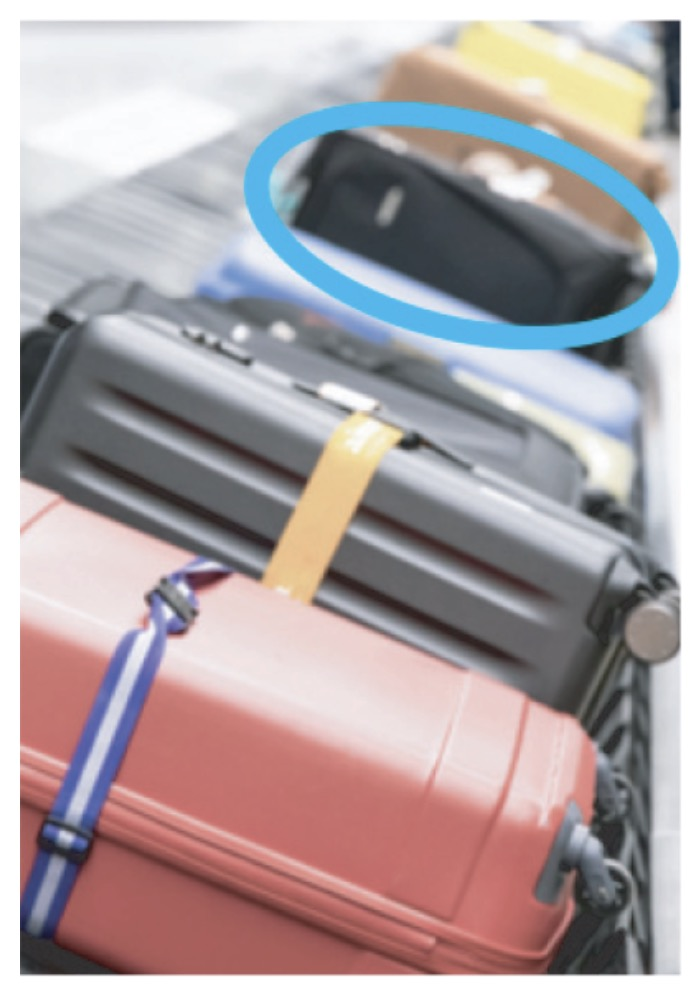
\includegraphics[width=3.75cm]{Bags.jpg}
\end{column}
% Right column: text
\begin{column}{0.66\textwidth}
\small
Let's suppose that you are an air traveler along with 99 other passengers from your flight, each of whom, like you, checked one item of luggage.

\vspace{0.2cm}
A recording piped through the speakers reminds you that:
\emph{``Many bags look alike. Please check your bag carefully before exiting the terminal.''}

\vspace{0.2cm}
Indeed, your bag is one of the most popular models on the market, a medium-sized black rectangular case \textbf{used by 5\% of all travelers}.

\vspace{0.2cm}
Given your distance from the luggage chute, you can discern only the shape, size, and color of the bags that emerge, not any detailed markings on the bags.
\end{column}
\end{columns}
\end{block}
\end{frame}

%-----------------------------------------------
\begin{frame}{}
\begin{block}{Question 9, cont.}
\begin{itemize}
\item[a.] Let's suppose that the \textbf{first bag} from your flight to enter the luggage carousel indeed has the same shape, size, and color as yours.
  Is it yours? Explain (i.e., calculate the posterior probability that the 1st bag is yours).
\vspace{0.4cm}
\item[b.] Now suppose that we continue to wait for our bag to appear, failing to see it among the first 98 bags to enter the carousel (i.e., only 2 bags are left to come off the airplane).
  Calculate the posterior probability that the \textbf{99th} bag, which also matches ours in shape, size, and color, is our own.
\end{itemize}
\vspace{0.4cm}
\small \alert{(maybe the answers will follow ...)}
\end{block}
\end{frame}

%-----------------------------------------------
\begin{frame}{}
\textbf{Answer: a.}
{\color{blue}
\footnotesize
Let \(Y\) = first bag is yours, and \(M\) = first bag matches.

\[
\begin{aligned}
&P(Y)=\frac{1}{100}\\
&\mathcal{L}(Y^c\mid M)=P(M\mid Y^c)=0.05\\
&\mathcal{L}(Y\mid M)=P(M\mid Y)=1\\
\end{aligned}
\]

\[
\begin{aligned}
P(Y\mid M)&=\frac{P(M\mid Y)P(Y)}{P(M)}
  =\frac{P(M\mid Y)P(Y)}
         {P(M\mid Y)P(Y)+P(M\mid Y^c)P(Y^c)}=\\
&=\frac{1\cdot 0.01}{1\cdot 0.01+0.05\cdot 0.99}
=\frac{0.01}{0.0595}\approx 0.168
\end{aligned}
\]

So even though the first bag matches, it is probably not yours.
}
\end{frame}

%-----------------------------------------------
\begin{frame}{}
\textbf{Answer: b.}
{\color{blue}
\footnotesize
\[
\begin{aligned}
P(Y\mid M)
&=\frac{1\cdot \tfrac{1}{\text{total of bags remaining}}}
{1\cdot \tfrac{1}{\text{total of bags remaining}} + 0.05\cdot \tfrac{\text{total of bags remaining} - 1}{\text{total of bags remaining}}}\\
&\text{(if 2 bags remain)}\\
&=\frac{1\cdot \tfrac{1}{2}}
{1\cdot \tfrac{1}{2} + 0.05\cdot \tfrac{1}{2}}=\frac{1}{1+0.05} \approx 0.9524
\end{aligned}
\]

There is a 95\% chance that the 99th bag is yours, given that it looks like yours.\\
Or, \hl{it is \textbf{19 times more likely} to be yours than not yours $^{(0.95/0.05 = 19)}$.}
}
\end{frame}
}

%-----------------------------------------------
\end{document}